\documentclass[a4paper]{article}
%\usepackage[left=3cm, right=3cm]{geometry}
\usepackage[utf8x]{inputenc}
\usepackage{float}
\usepackage{longtable}
\usepackage{hyperref}
\usepackage{cite}
\usepackage{amssymb}
\usepackage{amsmath}
\usepackage{url}
\usepackage{array}
\usepackage{algorithmic}
\usepackage[ruled]{algorithm}
\usepackage{color}
\usepackage{graphicx}
\usepackage{tabularx}
\usepackage{caption}
\usepackage{todonotes}
\usepackage{rotating}
\pagestyle{headings}
\newcommand{\secondo}{\textsc{Secondo}}
\newcommand{\bmodb} {BerlinMOD Benchmark}
\newcommand{\op}[1]{\textbf{#1}}
\newcommand{\dt}[1]{\textsl{\underline{#1}}}
\newcommand{\true}{\textsl{TRUE}}
\newcommand{\false}{\textsl{FALSE}}
%opening
\title{Network Data Model and BerlinMOD Benchmark}
\author{Simone Jandt}
\date{Last Update: \today}
\begin{document}
\maketitle
\begin{abstract}
In the past, several data models for the representation of histories of
spatio-temporal data objects have been developed. We can categorize these data
models
into data models for objects moving freely in the two dimensional space and data
models for network constrained moving objects. In this paper we select two
representatives,
one for each data model category, which are both implemented in the \secondo{} DBMS,
and compare their capabilities with the \bmodb{}. We describe our implementation
of the used network constrained data model, the translation
from the \bmodb{} into the network constrained data model, and show
that in our experiments the network constrained data model outperforms the data
model of free movement in the two dimensional space by orders of magnitude.
\end{abstract}
\section{Introduction}
In the past, several data models for the representation of
spatio-temporal data objects have been developed. We can categorize them into
data models for objects moving freely in two dimensional space (DMFS) and data
models
for network constrained moving objects (NCDM). For both categories several different
data models have been presented like
\cite{DataModelDataStructureGueting,RepresentingMovingObjectsGueting,STAUPelekis
,HERMESMDCPelekis}
for DMFS and
\cite{DynamicTransportNetworkDing,NetworkGueting,NetworkJensen,
NetworkVazirgiannis}
for NCDM, to name just a few. Objects which are restricted to use existing networks,
like cars are restricted to use road networks, can be represented as moving point
objects in both data models, whereas objects, which are not restricted by a given
network, like people, can be represented as moving point objects only in DMFS.

Why do we spend time on NCDM, if everything can be represented by DMFS?
Now, it is natural to give positions related to the street
network instead of coordinate pairs in the xy plane. NCDM are expected to use
less storage space,
because geographical information's about street curves are stored only once in
the network, whereas in DMFS each street curve is stored in each moving point
object using this street. NCDM can support query processing with specialized indexes
using their knowledge of the underlying network. It is much easier to
formulate queries about the relationships between moving objects and the network
in the NCDM. And not at last, the results of our experiments show that
our network constrained data model outperforms our data model of free movement in
two dimensional space by orders of magnitude. The network constrained data model
uses less than 60\% of the storage space and less than 50\% of the total query
run time of the data model of free movement in space, which we used in our
experiments.
We think that these results show that it is useful to develop specialized data
models for specialized data structures like NCDM for
network constrained moving objects to save storage space and reduce query run times.

For our benchmark experiments, presented in this paper, we chose two data models
one for each data model category. Both data models use the same temporal
representation
and are available in \secondo{} DBMS
\cite{SecondoEnvironmentDieker,SecondoPlatformPrototypingGueting}.
So we can exclude that different DBMS or temporal representation issues bias the
results of our data model comparison with the \bmodb{}\cite{BerlinMODVLDBDuentgen}.
The DMFS we use is the data model presented in
\cite{RepresentingMovingObjectsGueting,DataModelDataStructureGueting}
(SPACE). And the NCDM we use is the data model presented in
\cite{NetworkGueting} (NET).

We used the \bmodb{} \cite{BerlinMODVLDBDuentgen} to compare the capabilities of
the two data models, because the \bmodb{} is to the best of our knowledge the
first benchmark for complete spatio-temporal database systems.
It is developed and available in \secondo{} DBMS. And the data generated by the
\bmodb{} data generator are restricted to the streets of the German capital Berlin,
such that they can be translated into a network constrained environment.
And not at last, the data model used in the \bmodb{} is SPACE that we use
for our comparison. So we only have to translate the spatial and spatio-temporal
data types of the \bmodb{} once into our NET representation. This simplifies the
control of the query results and avoids errors caused by translation.
The translation of the spatial and spatio-temporal data types of the \bmodb{} data
into the NET representation described in Section \ref{sec:Translation} can be
seen as an example for the usage of the \bmodb{} with other compatible data
representations or DBMS.

Besides the comparsion of the both data models, we describe in this paper the
first real implementation of NET (see Section \ref{sec:implNDM}) providing some
further concepts which were only sketched in \cite{NetworkGueting}.

The rest of the paper is organised as follows: We present some related work in
Section
\ref{sec:relWork}, including short reviews of the underlying \secondo{} DBMS
(Section \ref{sec:secondo}), the two data models (SPACE Section
\ref{sec:bmodbdatamod},
NET Section \ref{sec:netdatamod}) we chose for our comparison, and the
\bmodb{} (Section \ref{sec:bmodb}).
In Section \ref{sec:implNDM} we give some information's about our implementation
of NET, the used operations and indexes.
The translation of the \bmodb{} data and query set into the NET representation
is described in Section \ref{sec:Translation}. The resulting experimental benchmark
setup is described in Section \ref{sec:scenario} followed by the results of our
experiments in Section \ref{sec:results}. We conclude our work in Section
\ref{sec:summary}.
\section{Related Work}
\label{sec:relWork}
In the past many different spatio-temporal data models have been presented. Many
of them support only discrete spatio-temporal changes like
\cite{sqlstchen,HunterWilliamson,Langran2,Langran1,Ramadrachan}
or deal only with current and future positions of continuously moving objects like
\cite{MOSTWolfson}. More detailed reviews of these and other spatio-temporal
data models beyond the scope of our paper can be found in \cite{ReviewSTDMPelekis}.

In this paper we will focus on spatio-temporal data models for complete histories
of continuously moving objects. These can be categorized into data models for
objects moving freely in two dimensional space (DMFS) and data models for network
constrained moving objects (NCDM).

\cite{MOLRaQSu} proposes an incomplete abstract DMFS. Basic idea is that
spatio-temporal data types can be modeled by linear constraints and queries
can be formulated using formulas from differential geometry.

\cite{RepresentingMovingObjectsGueting} proposes an abstract DMFS including the
idea of an time sliced representation for moving objects. This basic idea of
time sliced representation is used by the DMFS \cite{STAUPelekis} and
\cite{DataModelDataStructureGueting}. The last one is used in our experiments
and therefore reviewed in more detail in Section \ref{sec:bmodbdatamod}.
The main difference between the both data models is that
\cite{DataModelDataStructureGueting} supports only linear interpolation of movement,
whereas \cite{STAUPelekis} also supports arc interpolation of movement.
\cite{STAUPelekis} uses only one spatial object
containing all spatial geometries for the representation of spatial objects and
one moving object for the representation of the different moving object data types,
whereas \cite{DataModelDataStructureGueting} uses different spatial and moving
objects for the representation of the different spatial and moving data types.
According to this, \cite{STAUPelekis} provides only a single operator that
distinguishes
between the different topological relationships via a parameter, whereas
\cite{DataModelDataStructureGueting} uses different operations to estimate
topological relationships. Overall, \cite{STAUPelekis} offers a more flexible
object oriented design than \cite{DataModelDataStructureGueting}.

The spatio-temporal framework of \cite{RepresentingMovingObjectsGueting} used by
\cite{DataModelDataStructureGueting} has been used for the definition of a
NCDM in \cite{NetworkGueting}.

The most NCDM use edge based graph representations for the representation of the
underlying network data only a small number of NCDM use route oriented data
models or combine route and edge based data models.

\cite{NetworkVazirgiannis} proposes an edge based NCDM. The edges and their
attributes
are stored in a relation representing the network as an undirected graph. Moving
objects are assumed to drive always on the path with the lowest cost,
in terms of distance or travel-time. They are defined by the source point, the
target point, and the starting time instant of the trip. The trajectory is
computed by this assumption using the length and speed attributes of the graph
edges within the shortest, respectively, fastest path computation.
The advantage of this definition is the reduced storage space for the representation
of moving point objects. The drawback is the high computational effort for query
evaluation on moving objects.

\cite{NetworkJensen} uses also an edge based network representation. The paper
proposes a combination of an two dimensional geometrical edge representation with
an directed graph representation of the same network. The both representations
are connected by transition policies. The two dimensional
geometrical representation handles the spatial information's, whereas the
connectivity
information is mostly embedded in the directed graph representation.
Moving objects are represented by sets of five tuples. Each five tuple contains
an edge identifier, the position of the moving point on the edge
in terms of weight and length, the speed and direction of the movement, and
the time instant of this information.

Another two-layer network representation is proposed by
\cite{DynamicTransportNetworkDing}.
The authors of \cite{DynamicTransportNetworkDing} combine the advantages of the
dynamic edge-based \cite{DynNetworkModEdgeGueting} and the dynamic route-based
\cite{DynNetworkModRouteGueting} NCDM approaches. The route-based environment
reduces the update intervals and used storage space for the database representation
of moving point objects, whereas the edge-based environment supports
a more detailed view on the traffic conditions of the different edges belonging
to the same route. Moving objects are represented by a set of pairs. The pairs
consist of an motion vector and an Boolean flag. The Boolean flag tells if the
motion vector contains current or historical information. Each motion vector
consists, in parts similar to \cite{NetworkJensen}, of a time stamp, a network
position, and a speed vector. Similar to \cite{NetworkGueting} the network
positions are given related to routes and junctions and not on edges. Different
from all
other NCDM in this section \cite{DynamicTransportNetworkDing}
uses time depending dynamic attributes in the representation of the network parts.
Therefore, changes in the network environment can be handled without loss of
information in this NCDM.

To the best of our knowledge only a few of the proposed data models have been
implemented into database management systems: \cite{STAUPelekis} is implemented
as data cartridge \cite{HERMESMDCPelekis, HERMESPelekis} for the commercial
Oracle\textregistered{} object-relational DBMS \cite{oracle};
\cite{DynamicTransportNetworkDing} is implemented as extension of the open source
database project PostgreSQL \cite{PostgreSQL}; \cite{DataModelDataStructureGueting}
and \cite{NetworkGueting} are implemented in the freely available extensible
\secondo{} DBMS \cite{SecondoPlatformPrototypingGueting}.

Although \cite{STAUPelekis} for the DMFS and \cite{DynamicTransportNetworkDing} for
the NCDM provide greater flexibility we decided to use
\cite{DataModelDataStructureGueting} and \cite{NetworkGueting} in our
experiments, because both data models are available in the same DBMS, which is
also the DBMS in which the \bmodb{} \cite{BerlinMODVLDBDuentgen} has been
developed.

The \bmodb{} \cite{BerlinMODVLDBDuentgen} is to the best of our knowledge the only
benchmark testing the capabilities of complete spatio-temporal database systems.
Coming with a well defined data set, and two query sets feasible for DMFS and NCDM.
Other benchmarks for spatio-temporal databases systems provide only well defined
query sets and a database description without any data set like
\cite{QueriesTheodoridis}.
Or they come with well defined data generation, workload sets and experiments but
evaluate only the capabilties of indexes for current and near future positions like
\cite{COSTBenchmarkJensen}. Or they focus on time-evolving regional data and
associated
index methods like \cite{BenchmarkTzouramanis}.

The focus on index benchmarking in the most benchmarks is dued by the fact that
indexes have a great influence on query run times. Therefore, many spatio-temporal
indexes have been developed in the last ten years. An survey about existing
spatio-temporal
indexes can be found in the two parted work \cite{STAMSurvey1} and
\cite{STAMSurvey2}.
The most presented spatio-temporal indexes base on the R-Tree \cite{RTreeGuttmann}
and its variants. The R-Trees are used stand alone or in hierarchical combinations.
B-Trees \cite{BTreeBayer} and their variants are also used within spatio-temporal
indexes. \secondo{} comes with implementations of R-Tree, B-Tree, and MON-Tree
\cite{MONTreeAlmeidaGeoinformatica} in Section \ref{sec:implNDM} we give a detailed
description how we used these indexes in our experiments.

The \bmodb{} comes with his own data generator. Like mentioned before other
benchmarks like \cite{QueriesTheodoridis} define only database descriptions.
The users have to generate their own corresponding data.

Therefore, several data generators have been developed. Some of them generate
only unconstrained moving point objects like \cite{OportoSaglio}, or support
only short-term observations like \cite{BrinkhoffsDataGenerator}, or require
additional software like \cite{STACTS}.

In the sequel we give short reviews of the \secondo{} DBMS
(Section \ref{sec:secondo}), the both data models we used in our experiments
(Section \ref{sec:bmodbdatamod} and Section \ref{sec:netdatamod}), and the \bmodb{}
(Section \ref{sec:bmodb}).
\subsection{\secondo{} DBMS}
\label{sec:secondo}
The extensible \secondo{} DBMS presented in
\cite{SecondoEnvironmentDieker,SecondoPlatformPrototypingGueting} provides a
platform for implementing various kinds of data models. It provides a clean
interface between the data model independent system frame and the content of the
single data models. Hence \secondo{} can be easily extended by the user
implementing algebra modules to introduce new data types and operations on
these data types. The user may define additional viewers for the graphical user
interface or write additional optimization rules or cost functions to extend the
the optimizer. Since \secondo{} version 2.9 the users may publish their extensions
as a \secondo{} plugin such that other users can use these plugins to extend
their own
\secondo{} system. They may use the newly provided functionalities or repeat the
published experiments. \secondo{} is freely available on the web \cite{secondoweb}.
It comes with a number of already implemented spatial and spatio-temporal data types
and operations including SPACE (Section \ref{sec:bmodbdatamod}) and NET
(Section \ref{sec:netdatamod}). Furthermore, the \bmodb{}
described in Section \ref{sec:bmodb} has been developed in the \secondo{} DBMS.
For our experiments we used the \secondo{} version 3.0.
\subsection{Data Model of \bmodb{} (SPACE)}
\label{sec:bmodbdatamod}
\cite{STDTModelingQueryingMOinDErwig} presents the basic idea of the DMFS that
is used by the \bmodb{}. The abstract data model for SPACE was pubished in
\cite{RepresentingMovingObjectsGueting} and the discrete data model in
\cite{DataModelDataStructureGueting}. Abstract data models are useful as conceptual
models, but they cannot be implemented, because computers can only use finite sets.
In the sequel we will mainly focus on the discrete data model.

The type system in \cite{RepresentingMovingObjectsGueting} is defined using the
techniques presented in \cite{SecondOrderSignatureGueting}. The basic idea of
\cite{RepresentingMovingObjectsGueting} is to define type constructors
that create new data types if they are applied to an data type of a given set of
basic data types.

Basic data types are the standard data types integer, real, string and boolean
(BASE);
the spatial data types point, points, line, and region (SPATIAL);
and the temporal type instant (TIME).

The carrier sets for all data types in the discrete data model contain
$\{\perp\}$. $\perp$ represents an undefined value. 

The carrier sets for the BASE data types in the discrete data model are defined
by the corresponding programming language data types \dt{int}, \dt{real}, \dt{bool},
and \dt{string}. The carrier set of a value of the data type \dt{point} is
\dt{real} $\times$ \dt{real}. The two \dt{real} values represent the
coordinate pair of the position of the \dt{point} value in the xy plane. 

The data type \dt{points} consists of a disjoint set of \dt{point} values. 

The carrier set for the data type \dt{line}
consists of a finite set of disjoint line segments representing the linear
approximation of the line curve in the two dimensional plane. Semanticaly an
\dt{line} value is the union of the points of all its line segments. 

A region
is the union of all points covered by the region. The carrier set \dt{region}
is defined to be a finite set of line segments building a polygon representing
the linear approximation of the outer and, if the region contains wholes, inner
borders of the region. The borders are defined to belong to the region.

The carrier set for the TIME data type is given by \dt{real} in the discrete
data model.
That means each time \dt{instant} is represented by a corresponding \dt{real}
value.

The type constructor \dt{range} converts BASE and TIME data types $\alpha$ into
a type whoes values are finite sets of intervals over $\alpha$. Range types are
used to represent collections of time intervals, or the values taken by a moving
real. Intervals are represented by their start and end point and two flags
indicating if the start, respectively, end point is part of the interval or not.

The other important type constructor of the abstract data model is \dt{moving}.
In the abstract data model \dt{moving} maps each data type $\alpha$ from BASE
and
SPATIAL into an time dependend spatio-temporal moving data type
\dt{moving}($\alpha$)
(\dt{m$\alpha$} for short) of kind TEMPORAL. The discrete data model introduces some
additional type constructors to implement the moving type constructor of the
abstract data model. A detailed description of the type constructors is skiped
due to place limitations. We explain the realisation of \dt{moving} at the example
of a \dt{moving}(\dt{point}) (short \dt{mpoint}) object. An \dt{mpoint} value
may represent a car, which changes its position in the plain within time.

An \dt{mpoint} consists of a set of so called \dt{unit}(\dt{point}) values
(\dt{upoint} for short).
Each \dt{upoint} consists of a time interval and two \dt{point} values. The first
\dt{point} value represents the position of the \dt{upoint} at the start of the
time interval and the second \dt{point} value represents the position of the
\dt{upoint} at the end of the time interval. It is assumed that the object,
represented by the \dt{upoint}, moves on the straight line between these two
points with constant
speed within the given time interval. The velocity of the object is given by the
ratio from the distance of the two points and the length of the time interval of
the \dt{upoint}.

All \dt{upoint} values of an \dt{mpoint} must have disjoint time intervals,
because a car cannot be at two different positions at the same time.
The set of \dt{upoint} values is sorted by ascending time intervals.

This spatio-temporal data model of \dt{moving} allows us to compute the position
of an \dt{mpoint} at every time instant within its definition time.
We can also compute the time instant the point passed a
given position assuming the \dt{mpoint} ever passes this position. The position of a
\dt{point} at a given time instant is represented by an \dt{intime}(\dt{point})
(short form \dt{ipoint}). An \dt{ipoint} consists of an time instant and an
\dt{point}
value and represents the position of the \dt{mpoint} value at the given time
instant.

Other data types of \secondo{} which are used in the \bmodb{} are \dt{mbool},
\dt{mreal}, and \dt{periods}. A \dt{mbool} value consists of a set of \dt{ubool}
values. Each \dt{ubool} value is is constant \true{} or \false{} for the given
time interval. A \dt{mreal} value consists of a set of \dt{ureal} values. Each
\dt{ureal} value is defined by a function of time representing the \dt{real}
value at each time instant. A \dt{periods} value is a set of disjoint an not
connected time intervals.
\subsection{Network Data Model(NET)}
\label{sec:netdatamod}
The central idea of the network constrained data model NET presented in
\cite{NetworkGueting} is that
every movement is constrained by a given network and every position can be described
relative to this network. Contrary to the most other NCDM NET models the network
in terms of routes, corresponding to roads or highways in real life. Positions
are given by a route identifier and the distance from the start of the route.
This is a more natural representation of network positions as the directed graph
representation of networks, where junctions are vertexes and the pieces between
junctions are represented by edges, which is used in the most NCDM. We have names
for roads not for junctions or pieces between junctions.

The routes based network representation has the advantage that the
representation of moving objects that move over several sections of the same route
with constant speed becomes much smaller. We only have to store an new unit
if the moving object changes the route or the speed, not every time
it passes a junction like in the edge based NCDM.

In NET the data type \dt{network} is modeled by two main components. One is the
set  of routes (streets) and the other one the set of junctions (crossings). The
domain of routes is defined as
\[
\begin{split}
Route = \{(id,\ l,\ c,\ kind,\ start)\ &|\ id \in \dt{int},\ l \in \dt{real},
\ c \in \dt{line},\\
&\ kind \in \{simple,\ dual\},\\
&\ start \in \{smaller,\ larger\}\},
\end{split}
\]
where $id$ is a distinct route idenitfier, $l$ is the length of the route, $c$
is the route curve as \dt{line} value (see Section \ref{sec:bmodbdatamod}),
\textit{kind} indicates if the lanes of the route are separated, and \textit{start} indicates
how the route curve is embedded into space.

If $R$ is a set of distinct routes, the domain of junctions in $R$ is defined as
\[
  \begin{split}
    Junction(R)=\{(rm_1,\ rm_2,\ cc)\ &|\ rm_1,\ rm_2 \in RMeas(R),\\
&rm_1 = (r_1,\ d_1),\ rm_2 = (r_2,\ d_2),\\
&r_1 \neq r_2,\ cc \in \dt{int}\}.
  \end{split}
\]
Where the set of possible positions in $R$ $RMeas(R)$ is defined as
\[
  \begin{split}
    RMeas(R) = \{(rid, d)\ &|\ rid \in \dt{int},\ d \in \dt{real},\\
&\exists (rid,\ l,\ c,\ k,\ s) \in R \wedge 0 \leq d \leq l\},
  \end{split}
\]
where $d$ is the distance from the start of the route and the connectivity code
$cc$ encodes which lanes of the routes are connected
by the junction\footnote{See \cite{NetworkGueting} for a detailed
explanation of the different connectivity code values.}.

A network $N$ is a pair $(R,\ J)$, where $R$ is a finite set of distinct routes
and $J$ is a finite set of junctions in $R$. The carrier set for network
positions $Loc(N)$ is equal to the set of route locations $RLoc(R)$ and defined
as
\[
  \begin{split}
    RLoc(R)=\{(rid,\ d,\ side)\ &|\ (rid,\ d) \in RMeas(R),\\
&side \in \{up,\ down,\ none\}\}.
  \end{split}
\]
The \textit{side} value indicates for \textit{dual} routes if a position can be reached
from the \textit{up} or the \textit{down} side of the route. For routes of \textit{kind simple}
the \textit{side} value is always \textit{none}.

Let $N=\{N_1,\ldots,N_k\}$ be a set of networks. A single network position in a
network $N_i$ is represented by the data type \dt{gpoint}. The carrier set of
\dt{gpoint} is defined as
\[\{(i,\ gp)\ |\ 1 \leq i \leq k \wedge gp \in RLoc(R) \cup \{ \perp \}\},\]
where $\perp$ again represents an undefined value.

A \textit{route interval} in $N_i$ is a pair of network positions on the same
route. 
The \textit{route interval} is represented by a quadruple $(rid,\ d_1,\ d_2,\
side)$, with
$(rid,\ d_1,\ side),\ (rid,\ d_2,\ side) \in Loc(N)$
and $d_1 \leq d_2$. Semantically
a \textit{route interval} represents all route locations $(rid,\ d,\ side)$ with
$d_1 \leq d \leq d_2$. A finite set of disjoint \textit{route intervals} of a
network
$N_i$ is called region of $N_i$. The set of all possible regions in a network
$N_i$ is
denoted as $Reg(N_i)$.

A region within an network $N_i$ is represented by the data type \dt{gline}.
The carrier set of \dt{gline} is defined as
\[\{(i,\ gl)\ |\ 1 \leq i \leq k \wedge gl \in Reg(N_i) \} \cup \{\}\].
The set of \textit{route intervals} defining a network region may be empty.

The type systesm of \cite{RepresentingMovingObjectsGueting} is extended by
\cite{NetworkGueting} to contain a new kind GRAPH consisting of the data types
\dt{gpoint} and \dt{gline}. The type constructors \dt{moving} is also extended
to be feasible for data types of kind GRAPH. Therefore the data type
\dt{moving}(\dt{gpoint}) (\dt{mgpoint} for short) is defined similar to the
\dt{mpoint} explained in detail in Section \ref{sec:bmodbdatamod}. The units of
a \dt{mgpoint} consist of \dt{ugpoint} values and single positions of a
\dt{mgpoint} are be given by \dt{igpoint} values.

The paper provides numerous operations on the network and the network data
types.
We give reviews of the operations that were use in our experiments later in
Section \ref{sec:implNDM} and Section \ref{sec:Translation}.

\cite{NetworkGueting} proposes also implementational issues for NET in
\secondo{}. The implementation of the data type \dt{network} consists of three
relations called \textit{routes}, \textit{junctions}, and \textit{sections}, and a persistent
adjacency
list data structure supporting trip and path computations.

The three relations have the following schemas:
\begin{ttfamily}
\begin{itemize}
  \item [] routes (id: int; length: real; curve: line; kind: bool;\\
 start: bool)
  \item [] junctions (r1id: int; r1rc: int; pos1: real; r2id: int;\\
r2rc: int; pos2: real; cc: int; pos: point)
  \item [] sections (rid: int; rrc: int; pos1: real; pos2: real;\\
dual: bool; length: real; curve: line)
\end{itemize}
\end{ttfamily}
As you can see, the \textit{routes} relation is equivalent to the domain of routes
$Route$.
The tuple of the \textit{junctions} relation is somewhat different from $Junctions(R)$.
The record identifiers $r1rc$ and $r2rc$ support faster access to the
corresponding
tuples in the \textit{routes} relation and the \dt{point} value $pos$ supports the
connection
to the two dimensional plane.

The \textit{sections} relation is derived from the other two relations. The meaning of
the $rrc$ value is similar to the meaning of $r1rc$ in the \textit{junctions} relation.
The entries of the \textit{sections} relation correspond to the edges of a network
graph.
They are used internally to support operations like \op{shortestpath}. The
adjacency
list data structure consists of two arrays and provides a fast
access from each section to their adjacent sections with respect to the driving
direction. Two sections are adjacent if their lanes are connected by a junction.

For the data types \dt{gpoint} and \dt{gline} \cite{NetworkGueting} proposes
the following implementations:
\begin{ttfamily}
\begin{itemize}
  \item [] gpoint: record \{nid: int; rid: int; pos: real;\\
side: \{up, down, none\};\}
  \item [] gline: record\{nid: int; rints: DBArray of record \{\\
rid: int; pos1: real; pos2: real;\\
side: \{up, down, none\};\};\}
\end{itemize}
\end{ttfamily}
For the data type \dt{mgpoint} the implementation consists of a set of
\dt{ugpoint}.
The set is stored in a DBArray in ascending order of the time intervals of the
\dt{ugpoint}. Each \dt{ugpoint} is defined as:
\begin{ttfamily}
\begin{itemize}
  \item [] ugpoint: record \{nid: int; rid: int; pos1: real;\\
pos2: real; side: \{up, down, none\};\\
t1: Instant; t2: Instant;\}
\end{itemize}
\end{ttfamily}
The \dt{ugpoint} is expected to move from $pos_1$ to $pos_2$ with constant speed
on
route $rid$ in the given network $nid$ within the time interval defined by $t_1$
and $t_2$. Every time a \dt{mgpoint} changes the speed or changes the route a
new
\dt{ugpoint} is written.

We extended this implementation proposed by \cite{NetworkGueting} within our
experiments to support faster query execution. Our changes will be described in
detail in Section \ref{sec:implNDM}.
\subsection{BerlinMOD Benchmark}
\label{sec:bmodb}
The \bmodb{} was presented in \cite{BerlinMODVLDBDuentgen} and the
provided scripts for the data generator are implemented as \secondo{} DBMS
operations.
The \bmodb{} is available on the web \cite{berlinmodweb} and provides a well
defined
data-set and queries for the experimental evaluation of the capabilities of
spatial and spatio-temporal database systems dealing with histories of moving
objects. The \bmodb{} emphasises the development of complete systems
and simplifies experimental repeatability pointing out the capabilities and the
weaknesses of the benchmarked systems.

The data-sets of the \bmodb{} are created using the street map of the German
capital Berlin \cite{bbike} and statistical data about the regions of Berlin
\cite{bevberlin,berlinstadtatlas} as input relations.
The created moving objects represent cars driving in the streets of Berlin,
simulating the behaviour of people living and working in Berlin.
Every moving object has a home node and a work node. Every weekday each car will
do a trip from the home node to the work node in the morning and vice versa
in the late afternoon. Beside this, randomly chosen cars will make additional
trips in the evening and up to six times at the weekend to randomly chosen
targets in Berlin and back home. The \bmodb{} uses the data model of free
movement in two dimensional space described in Section \ref{sec:bmodbdatamod}.
Because the \bmodb{} generates all data sets restricted to the street map of
Berlin, the \bmodb{} can also be used for network constrained data models, if
the spatial and spatio-temporal data types are translated into a corresponding
NCDM, like we did for our experiments.

The number of observed cars and the duration of the observation period can be
influenced by the user setting the \textit{scalefactor} to different values in
the data
generation script of the \bmodb{}. For example at \textit{scalefactor} 1.0 the
data
generator creates 2000 moving point objects observed for 28 days, each of them
sending a GPS-signal every 2 seconds. These simulated signals are simplified
such that time intervals when a car does not move or moves in the same direction
at the same speed are merged into one single time interval. For example: If a
car is parked in front of the work node for 8 hours, there will be only one
entry in the history of the cars movement with a time interval of 8 hours
instead of 14.400 entries, one for each GPS time interval.

The \bmodb{} provides two different approaches to store the histories of moving
objects, called the object-based approach (OBA) and the trip based approach
(TBA),
respectively.

In the OBA, the complete history for each moving object is kept together in one
single entry. There is only one relation \textit{dataScar}
containing one tuple for each object consisting of the spatio-temporal data of
the object \textit{trip} (\dt{mgpoint}), the \textit{licence}, the \textit{type}, and the \textit{model}
of the object (all \dt{string}).

In the TBA, we have two relations \textit{dataMcar} and \textit{dataMtrip}.
\textit{dataMcar} contains
the static data for each object like \textit{licence}, \textit{type}, and \textit{model} together
with an object identifier \textit{moid} (\dt{int}). \textit{dataMtrip} contains for
each \textit{moid} several tuples, each of them containing either all units of a single
trip of the moving object, or a single unit for a longer stop. For example, each
time the car drives from home node to work node is a single trip, and each time
the car is parked in front of the office is also a single trip.

Besides the moving point objects, the \bmodb{} provides several data sets, each
of them containing 100 pseudo randomly generated data objects, which are used in
the benchmark queries. Table \ref{tab:queryobjects} gives an overview of these
query objects. The \bmodb{} deals also with subsets from these query object
sets consisting of the first or second 10 query objects of a query object set.
They are labeled by the name of the query object set followed by a 1 for the
first ten or a 2 for the second ten query objects.

\begin{table}[htbp]
  \begin{tabularx}{1.0\textwidth}{|l|X|}
    \hline
    \textbf{Name of Data Set}&\textbf{Tuple Content}\\
    \hline
    \textit{QueryPoints}   & Object identifier and \dt{point} value\\
    \hline
    \textit{QueryRegions}  & Object identifier and \dt{region} value\\
    \hline
    \textit{QueryInstants} & Object identifier and time instant\\
    \hline
    \textit{QueryPeriods}  & Object identifier and time interval\\
    \hline
    \textit{QueryLicences} & Object identifier and a \dt{string} representing a
licence value\\
    \hline
  \end{tabularx}
  \caption{Query Object Relations of \bmodb{}}
  \label{tab:queryobjects}
\end{table}

The \bmodb{} provides two sets of queries BerlinMOD/R and BerlinMOD/NN.
BerlinMOD/R addresses range queries and BerlinMOD/NN nearest neighbour queries.
In this paper we will focus on the range queries, which are the main aspect of
the
\bmodb{} up to now.

The query set BerlinMOD/R includes 17 queries selected of the set of possible
combinations of the 5 aspects:
\begin{itemize}
  \item known or unknown object identity,
  \item standard attribute, spatial, temporal, or spatio-temporal dimension,
  \item point, range, or unbounded query interval,
  \item single object or object relationships condition type,
  \item with or without aggregation.
\end{itemize}
We will present the 17 queries in more detail in Section
\ref{sec:queries} together with our NET algorithms for these queries.
\section{Implementation of NET}
\label{sec:implNDM}
In Section \ref{sec:netdatamod} we described the implementation of NET
provided by \cite{NetworkGueting}. The provided implementation
has been changed and extended by us at some points to support faster query
execution. In this section we describe the current implementation of the NET
data structure and data types in \secondo{} DBMS. In Section
\ref{sec:implNetDataTyp} we present our implementation of the NET data
types. In Section \ref{sec:implNetIndex} we introduce so called
(temporal) network bounding boxes that can be used in R-Trees to index
(temporal) network positions. In Section \ref{sec:implNetOperations} we
describe the implementation of NET operations used by the \bmodb{}.
\subsection{Data Type Implementation}
\label{sec:implNetDataTyp}
First of all the \dt{network} object itself has been changed. The \textit{junctions}
relation has been extended by four additional record identifiers, one for each
section connected within this junction. Four B-Tree indexes for the route
identifier attributes in the \textit{routes}, \textit{junctions}, and \textit{sections} relations
have been integrated in the data type \dt{network}. An R-Tree has been
integrated indexing the \textit{route curve} attribute
of the \textit{routes} relation. All this has been done to support faster access to
spatial routes data in query evaluation.

The \textit{side} value of the \textit{route intervals} is not yet part of the
implementation.

\label{sec:sortedgline}
The record of \dt{gline} was extended by an attribute \textit{length} of
\dt{real}, storing the length of the \dt{gline}, and an sorted flag, indicating
if the \textit{route intervals} in the DBArray are stored sorted or not. We call
a
set of \textit{route intervals} sorted if it fullfills the following conditions:
\begin{itemize}
   \item all \textit{route intervals} are disjoint
   \item the \textit{route intervals} are stored in ascending order of their
route identifiers ($rid$)
   \item if two \textit{route intervals} have the same route identifier ($rid$),
the
\textit{route interval} with the smaller start position $d_1$ is stored first if
the
\textit{route intervals} are disjoint
   \item for all \textit{route intervals}, $start\ position \le end\ position$
\end{itemize}
We introduced this definition and the sorted flag, because many algorithms take
profit
from sorted \dt{gline} values. Let $r$ be the number of \textit{route intervals}
in a
\dt{gline}, the decision, if a \dt{gpoint} is inside the \dt{gline} needs O($r$)
time for unsorted and O($\log r$) time for sorted \dt{gline} values.

Unfortunately not all \dt{gline} values can be stored sorted. If a \dt{gline}
value represents a path between two \dt{gpoint} in the network, we need the
route intervals exactly in the sequence they are used in the path. This will
nearly never be a sorted set like defined before.  We store \dt{gline}
values sorted whenever this is possible to support faster query execution.
Every algorithm which deals with \dt{gline} values checks this flag and uses
the corresponding code.

For sorting and compressing \textit{route intervals} we introduced a binary tree
data structure called \textit{RITree}. This \textit{RITree} sorts and compresses the inserted
\textit{route intervals}. If $r_i$ is the number of inserted \textit{route
intervals} and
$r_{res}$ the number of resulting \textit{route intervals} sorting and
compressing takes
O($r_i \log r_{res}$) time. The sorted \textit{route intervals} are returned in
O($r_{res}$) time. We think that this time is well invested, because the sorted
\dt{gline} is computed once, but many different algorithms can be executed
faster
for sorted \dt{gline} values.

The implementation of the \dt{ugpoint} has been changed to:
\begin{ttfamily}
\begin{itemize}
  \item []ugpoint: record \{gp1: gpoint; gp2: gpoint; ti : Interval;\}
\end{itemize}
\end{ttfamily}
Where $t_i$ is a time interval consisting of two time instants $t_1$ and $t_2$
and
two Boolean flags, indicating if $t_1$ respectively $t_2$ is part of the time
interval
or not.

At the same time the implementation of \dt{mgpoint} has been extended to:
\begin{ttfamily}
\begin{itemize}
  \item [] mgpoint: record \{units: DBArray of ugpoint;\\
drivenDist: real; trajDefined: bool; mbr: rectangle3D\\
trajectory: DBArray of sorted \textit{route intervals};\}
\end{itemize}
\end{ttfamily}
The DBArray of \dt{ugpoint} is the same as in the data model of
\cite{NetworkGueting}.
The $drivenDist$ is the total length of all \dt{ugpoint} in the \dt{mgpoint}.
The DBArray of \textit{route intervals} represents all network positions ever
traversed
by the \dt{mgpoint}. The flag indicates if the \textit{trajectory} is well defined,
because this attribute is not maintenanced in every operation changing
\dt{mgpoint} values. And the minimum spatio-temporal bounding box $mbr$ can be
used for a preselection in spatio-temporal queries.

Why this extensions?
Now, analogous to sorted \dt{gline} values the \textit{trajectory} value makes it much
faster to decide whether an \dt{mgpoint} ever passed a given network position or
not. Instead of a linear check of all $m$ units of an \dt{mgpoint} we can
perform
a binary scan on the much smaller number $r$ of the passed \textit{route
intervals}.
This reduces the time complexity from O($m$) to O($\log r$) for operations
like \op{passes}.

The spatio-temporal minimum bounding box was introduced as an attribute to the
\dt{mgpoint} because the computation of this value is very expensive in NET.
Although each unit of an \dt{mgpoint} stays on the same route
at the same speed it may follow different spatial directions. For example, a
route may lead uphill in serpentine. A spatial bounding box only computed from
the spatial start and end position may not enclose all spatial positions of the
car within the unit. Therefore we always have to examine the spatial dimensions
of the \textit{route interval} passed within a unit to compute the units
bounding box
using Algorithm \ref{alg:unitbbox}.
\begin{algorithm}[H]
  \caption{Computation Spatio-Temporal Unit Bounding Box}
  \label{alg:unitbbox}
  \begin{algorithmic}[1]
    \STATE Get \textit{route curve} for $rid$ using B-Tree index of \textit{routes}
relation
    \STATE Extract subline of unit from \textit{route curve}
    \STATE Compute bounding box of subline
    \STATE Add time dimension from unit time interval
  \end{algorithmic}
\end{algorithm}
If the number of routes in the \textit{routes} relation is $R$ the first step has a
time complexity of O($\log R$) time. If the \textit{route curve} $r_i$ consists
of $l_i$
line segments the time complexity of step 2 and 3 is O($l_i$) in the worst case.
Step 4 is done in O(1) time. Together we get a time complexity of
O($\log {R} + l_i$) to compute the bounding box of a single unit.

To compute the $mbr$ this computation must be done for each of the $m$ units of
the \dt{mgpoint} value. Therefore the time complexity to compute a $mbr$ is 
O($m \log {R} + \sum_{i=1}^{m}{l_i}$).

The time complexity can be reduced if the \textit{trajectory} is defined. We can use
the $r$ \textit{route intervals} of the \textit{trajectory} similar to the $m$ units of
the \dt{mgpoint} to compute the spatial bounding box. The third dimension can be
added using the start and the end time instant of the \dt{mgpoint} value. This a
algorithm has a time complexity of O($r \log {R} + \sum_{i=1}^{r}{l_i}$), with
$r \ll m$ in nearly all cases.

But the computation is still expensive. So the $mbr$ is only computed on demand
or if we can get it for free. For example we can copy
the bounding box of an \dt{mpoint} at the translation time into an \dt{mgpoint}
in O(1) time.
Analogous to the \textit{trajectory} the $mbr$ is not maintained. If
the \dt{mgpoint} value changes, the $mbr$ is set to be undefined until
recomputing
is necessary.

\subsection{Network Environment Indexes}
\label{sec:implNetIndex}
Spatial and spatio-temporal bounding boxes are used to support spatial
and spatio-temporal indexing of spatial, respectively, spatio-temporal
positions.
Because of the special problems with spatio-temporal bounding boxes in network
environments (see Section \ref{sec:implNetDataTyp}) we use only for the trip
based approach a spatio-temporal bounding box tree
\textit{dataMNtrip\_SpatioTemp} and
this tree only indexes spatio-temporal bounding boxes for complete \dt{mgpoint}
values. In our experimental evaluation we also tried the MON-Tree 
\cite{MONTreeAlmeidaGeoinformatica} and more
detailed spatio-temporal unit bounding box R-Trees, but they all haven been
outperformed within our experimental evaluation of the network implementation
for the \bmodb{}.

We introduced Network Bounding Boxes (NBB) and Temporal Network Bounding Boxes
(TNBB) in our implementation to support indexing in terms of network positions
with R-Trees instead of spatial indexing.

Let \dt{ugpoint} and \textit{route interval} be defined like in
\ref{sec:netdatamod}.
The NBB of a \textit{route interval} is a degenerated two dimensional
rectangle $(rid,\ rid,\ d_1,\ d_2)$. Analogous the TNBB of a \dt{ugpoint}
value is a degenrated three dimensional rectangle $(rid,\ rid,\ d_1,\ d_2,\
t_1,\ t_2)$.

We use these NBB and TNBB to create R-Trees indexing the network
positions (NPI) and temporal network positions (TNPI) of the \dt{mgpoint} values
of the \bmodb{}. The NPI is created from the NBB of the \textit{route
intervals} of the \textit{trajectory} attribute of the \dt{mgpoint} values. And the
TNPI is created from the TNBB of the \dt{ugpoint} values of the \dt{mgpoint}
values.
\subsection{Network Operations used in \bmodb{}}
\label{sec:implNetOperations}
The operations used to construct an \dt{network} object, and
to translate spatial and spatio-temporal values into network values are
described in Section \ref{sec:Translation}. In this section we give an overview
of the operations on network objects used in the benchmark queries of the
\bmodb{}.

Let $m$ be the number of units of the \dt{mgpoint} value, $r$ (resp.
$r_1$, $r_2$) the number of \textit{route intervals} of a \dt{gline} value or
the \textit{trajectory} attribute of an \dt{mgpoint} value (resp. of the first, second
argument), $R$ the number of routes in the \dt{network} object, $l_i$ the
number of line segments of a route curve $rc_i$, and $p$ the number of time
intervals in a \dt{periods} value.

Table \ref{tab:simplenetoperations} gives an overview of the simple
operations for the NET representation of the \bmodb{}.
\begin{sidewaystable}
  \caption{Simple NET Operations}
  \label{tab:simplenetoperations}
  %\begin{scriptsize}
  \begin{center}
  \begin{tabularx}{1.0\textwidth}{|l|l|X|X|}
  \hline
  \textbf{Name}       & \textbf{Signature}                       & \textbf{Explanation}                         & \textbf{Complexity}\\
  \hline
  \op{routes  }       & \dt{network} $\rightarrow$ \dt{relation} & Returns the \textit{routes} relation of the \dt{network} object & O($R$)\\
  \hline
  \op{no\_components} & \dt{mgpoint} $\rightarrow$ \dt{real}     & Returns the number of units of the \dt{mgpoint}  & O(1)\\
  \hline
  \op{length}         & \dt{mgpoint} $\rightarrow$ \dt{real}     & Returns the driven distance of the \dt{mgpoint} & O(1)\\
  \hline
  \op{trajectory}     & \dt{mgpoint} $\rightarrow$ \dt{gline}    & Returns the \textit{trajectory} of the \dt{mgpoint} value as sorted \dt{gline} & O($m \log r + r$) if \textit{trajectory} is defined, O($r$) otherwise\\
  \hline
  \op{units}          & \dt{mgpoint} $\rightarrow$ \dt{stream}(\dt{ugpoint}) & Returns the \dt{ugpoint} values of the \dt{mgpoint} value as stream & O($m$)\\
  \hline
  \op{initial}        & \dt{mgpoint} $\rightarrow$ \dt{igpoint} & Returns the first position and the start time of the \dt{mgpoint} value & O(1)\\
  \hline
  \op{atinstant}      & \dt{mgpoint} $\times$ \dt{instant} $\rightarrow$ \dt{igpoint} & Returns the network position of the \dt{mgpoint} value at the given time instant & O($\log m$)\\
  \hline
  \op{val}            & \dt{igpoint} $\rightarrow$ \dt{gpoint}  & Returns the network position of the \dt{igpoint} value & O(1)\\
  \hline
  \op{inst}           & \dt{igpoint} $\rightarrow$ \dt{instant} & Returns the time instant of the \dt{igpoint} value & O(1)\\
  \hline
  \op{isempty}        & \dt{gline} $\rightarrow$ \dt{bool}      & Returns \true{} if the \dt{gline} has no \textit{route intervals} &  O(1)\\
  \hline
  \op{routeintervals} & \dt{gline} $\rightarrow$ \dt{stream}(\dt{rectangle}) & Returns the NBB for each \textit{route interval} of the \dt{gline} value in a stream & O($r$)\\
  \hline
  \op{gpoint2rect}    & \dt{gpoint} $\rightarrow$ \dt{rectangle} & Returns the NBB of the \dt{gpoint} value       & O(1)\\
\hline
  \op{unitbox}        & \dt{ugpoint} $\rightarrow$ \dt{rectangle3D} & Returns the TNBB of the \dt{ugpoint} value  & O(1)\\
  \hline
  \end{tabularx}
  \end{center}
  %\end{scriptsize}
\end{sidewaystable}

In the trip based approach (TBA) the result values of the different trips must
be
aggregated to an single result value. Therefore the operation \op{union} was
introduced. \op{union} gets two \dt{gline} values, respectively, two
\dt{mgpoint} values as
input and mixes them up to an single sorted \dt{gline}, respectively,
\dt{mgpoint} value.
\begin{tabbing}
xxxxxxxxxxxxxxxxxxxxxxxxxxxxxx\=xxxxxxxxxxxxxxxxxxxxxxxxxxxxxxxxxxx\kill
\dt{gline} $\times$ \dt{gline} $\rightarrow$ \dt{gline} \> $gline1$ \op{union}
$gline2$ \\
\dt{mgpoint} $\times$ \dt{mgpoint} $\rightarrow$ \dt{mgpoint} \> $mgpoint1$
\op{union} $mgpoint2$\\
\end{tabbing}
\begin{algorithm}[H]
  \caption{\op{union}($gl_1$, $gl_2$)}
  \label{alg:uniongline}
  \begin{algorithmic}[1]
    \IF{$gl_1$ is sorted AND $gl_2$ is sorted}
      \STATE Perform parallel scan of $gl_1$ and $gl_2$
      \IF{Current \textit{route intervals} do not intersect}
         \STATE Add smaller \textit{route interval} to $result$
         \STATE Continue Scan with next \textit{route interval}
      \ELSE
          \STATE Merge \textit{route intervals} into one
          \IF{Next \textit{route intervals} intersect the merged one}
            \STATE merge them too
          \ENDIF
          \STATE Add merged \textit{route interval} to $result$
          \STATE Continue Scan
      \ENDIF
    \ELSE
      \FOR{Each $route\ interval$ of $gl_1$ and $gl_2$}
        \STATE Insert \textit{route interval} into \textit{RITree}
      \ENDFOR
      \STATE Copy sorted \textit{route intervals} from \textit{RITree} to $result$
    \ENDIF
    \RETURN $result$
  \end{algorithmic}
\end{algorithm}
The Algorithm \ref{alg:uniongline} distinguishes between two cases:
If both \dt{gline} values are sorted (line 2 to line 13) the algorithm has a
time complexity of O($r_1 + r_2$). If one or both \dt{gline} are not sorted
(line 15 to line 18) the time complexity is O($(r_1 + r_2) \log r_{res} +
r_{res}$), if $r_{res}$ is the number of \textit{route intervals} of the
resulting \dt{gline}. The additional
time results from sorting and compressing the resulting \textit{route
intervals}. As mentioned before (see Section \ref{sec:implNetDataTyp}) we think
that this time is well invested, because many algorithms take profit from
sorted \dt{gline} values.

The computation of the union of two \dt{mgpoint} values works almost similar to
the \op{union} operation for two sorted \dt{gline}. We perform a parallel scan
through the \dt{mgpoint} values and add the units in the sequel of their time
intervals to the resulting \dt{mgpoint} value. If two units have overlapping
time
intervals and the positions of the \dt{ugpoint}s within the overlapping time
interval are not the same the resulting \dt{mgpoint} is not defined, otherwise
one unit is added to the result for the overlapping time interval. The time
complexity of the \op{union} operation is O($m_1 + m_2$).

\begin{tabbing}
xxxxxxxxxxxxxxxxxxxxxxxxxxxxxx\=xxxxxxxxxxxxxxxxxxxxxxxxxxxxxxxxxxx\kill
\dt{mgpoint} $\rightarrow$ \dt{rect3} \> \op{mgpbbox}($mgpoint$)\\
\end{tabbing}
The operation \op{mgpbbox} returns the spatio-temporal bounding box of an
\dt{mgpoint} value. As explained before (see Section \ref{sec:implNetDataTyp})
the $mbr$ value is not maintained such that the operation \op{mgpbbox} knows
three different cases:
\begin{enumerate}
  \item If the $mbr$ is defined it can be returned in O(1) time.
  \item The $mbr$ is not defined but the \textit{trajectory} can be used to compute the
$mbr$ the time complexity is O($r \log {R} + \sum_{i=1}^{r}{l_i}$)
  \item If the $mbr$ and \textit{trajectory} are not defined the time complexity will
be
O($m \log {R} + \sum_{i=1}^{m}{l_i}$)
\end{enumerate}

\begin{tabbing}
xxxxxxxxxxxxxxxxxxxxxxxxxxxxxx\=xxxxxxxxxxxxxxxxxxxxxxxxxxxxxxxxxxx\kill
\dt{mgpoint} $\times$ \dt{periods} $\rightarrow$ \dt{mgpoint} \> $mgpoint$
\op{atperiods} $periods$\\
\end{tabbing}
The operation \op{atperiods} restricts a \dt{mgpoint} value to the given
periods. The operation performs a binary scan of the units of the \dt{mgpoint}
to find the unit including the start time instant of the periods value,
respectively the last unit with an time interval smaller than the start time
instant of the periods value in O($\log m$) time. From that position the $k_i$
units, which have time intervals that intersect with the periods value are
copied to the result in O($k_i$) time\footnote{The first and last time
interval might be splitted at the start (resp. end) time instant of the periods
value in O(1) time.}. The total time complexity of the operation is O($\log {m}
+ k_i$)
\begin{tabbing}
xxxxxxxxxxxxxxxxxxxxxxxxxxxxxx\=xxxxxxxxxxxxxxxxxxxxxxxxxxxxxxxxxxx\kill
\dt{mgpoint} $\times$ \dt{periods} $\rightarrow$ \dt{bool} \> $mgpoint$
\op{present} $periods$\\
\end{tabbing}
The operation \op{present} returns \true{} if the \dt{mgpoint} value is
defined at least at one time instant inside the given \dt{Periods} value. The
algorithm works almost similar to the \op{atperiods} operation, but
the scan of the \dt{mgpoint} units is stopped immediately if a intersecting unit
is found. The worst case time complexity for the operation is O($\log {m}$).

For the Euclidean Distance computation we retranslate our network values into
spatial (\op{gline2line}) respectively spatio-temporal (\op{mgpoint2mpoint})
values. In \cite{NetworkGueting} all these operations are called \op{in\_space}.
\begin{tabbing}
xxxxxxxxxxxxxxxxxxxxxxxxxxxxxx\=xxxxxxxxxxxxxxxxxxxxxxxxxxxxxxxxxxx\kill
\dt{gline} $\rightarrow$ \dt{line} \> \op{gline2line}($gline$) \\
\dt{mgpoint} $\rightarrow$ \dt{mpoint} \> \op{mgpoint2mpoint}($mgpoint$)\\
\end{tabbing}
The operation \op{gline2line} uses Algorithm \ref{alg:gline2line} to
translate an \dt{gline} value into an \dt{line} value.
\begin{algorithm}[H]
  \caption{\op{gline2line}($gl$)}
  \label{alg:gline2line}
  \begin{algorithmic}[1]
    \FOR {each \textit{route interval} $ri$ of $gl$}
      \STATE Get \textit{route curve} $rc$ of $ri$ using
B-Tree index of \textit{routes} relation
      \STATE Perform binary search on the line segments of $rc$ to find $d_1$ of
$ri$
      \STATE Copy line segments to result $line$ until $d_2$ of $ri$ is reached.
    \ENDFOR
    \RETURN $line$
  \end{algorithmic}
\end{algorithm}
The loop from line 1 to
line 5 is repeated $r$ times. The B-Tree search in line 2 takes O($\log{R}$)
time. The binary search in line 3 takes O($\log l_i$) time. The copy operation
in line 4 takes in the worst case O($l_i$) time. The return of
the result has a worst case time complexity of O($\sum_{i=1}^{r}{l_i}$). For the
whole algorithm we
get
\[O(r \log{R} + \sum_{i=1}^{r}{\log{l_i}} + 2\sum_{i=1}^{r}{l_i})
= O(r \log{R} + \sum_{i=1}^{r}{l_i}).\]

The operation \op{mgpoint2mpoint} is described by Algorithm
\ref{alg:mgpoint2mpoint}. The loop from line 3 to line 28 is repeated $m$ times.
The statements from
line 5 to line 8 has a worst case time complexity from O($\log R + l_i$). But
these lines are only executed if the car enters a new \textit{route curve}.
We have three different cases for the computing of the $mpoint$ units. The
two simple cases from line 10 to line 11 and line 13 to line 16 have a time
complexity of O(1).
The third case (line 18 to line 25) has a worst case time complexity from
O($l_i$). The last line 29 has a time complexity of O($m_{res}$) if $m_{res}$ is
the number of units of the resulting \dt{mpoint} value. In the worst case we get
a time complexity for Algorithm \ref{alg:mgpoint2mpoint} of 
\[O(m \log {R} + \sum_{i=1}^{m}{l_i} + m_{res}).\]
\begin{algorithm}[H]
  \caption{\op{mgpoint2mpoint}($mgp$)}
  \label{alg:mgpoint2mpoint}
  \begin{algorithmic}[1]
    \STATE $actRID$ = -1
    \STATE Initialize resulting $mpoint$
    \FOR{each unit $curUGP$ of $mgp$}
      \IF{not (rid from $curUGP$ == $actRID$)}
        \STATE $actRID$ = $rid$ from $curUGP$
        \STATE $rc$ = \textit{route curve} of $actRID$
        \COMMENT{$rc$ determined using B-Tree Index of \textit{routes} relation}
        \STATE Perform binary search on the line segments of $rc$ to find
        line segment $l$ with $gp1$ of $curUGP$
        \STATE $upstart$ = x,y-coordinates of $gp1$
      \ENDIF
      \IF{$gp1$ = $gp2$}
        \STATE add unit $upstart,\ upstart$ to $mpoint$
      \ELSE
        \IF{$gp2$ is on $l$}
          \STATE $upend$ = x,y-coordinates of $gp2$
          \STATE add unit $upstart,\ upend$ to $mpoint$
          \STATE $upstart$ = $upend$
        \ELSE
          \STATE Follow $rc$ in moving direction of $curUGP$
          \WHILE{not($gp2$ is on $l$)}
            \STATE add unit from $upstart$ to $segment\ end\ position$ to
$mpoint$
            \STATE $upstart$ = $segment\ end\ position$
            \STATE $l$ = next line segment of $rc$ in moving direction
          \ENDWHILE
          \STATE $upend$ = x,y-coordinates of $gp2$
          \STATE add unit from $upstart$ to $upend$ to $mpoint$
        \ENDIF
      \ENDIF
    \ENDFOR
    \RETURN $mpoint$
  \end{algorithmic}
\end{algorithm}

\begin{tabbing}
xxxxxxxxxxxxxxxxxxxxxxxxxxxxxx\=xxxxxxxxxxxxxxxxxxxxxxxxxxxxxxxxxxx\kill
\dt{gline} $\times$ \dt{gline} $\rightarrow$ \dt{bool} \>
\op{intersects}($gline1$, $gline2$)\\
\end{tabbing}
The operation \op{intersects} returns \true{} if two \dt{gline} values
intersect, \false{} otherwise. The Algorithm \ref{alg:intersectsgline} for
\op{intersects} differentiates three cases:
\begin{enumerate}
\item If both \dt{gline} values are sorted (see line 2 to line 5) the time
complexity
is O($r_1 + r_2)$)
\item If both \dt{gline} values are not sorted (see line 8 to line 14) the time
complexity is O($r_1r_2$)
\item If only one \dt{gline} value is sorted (see line 16 to
line 21) the time complexity is O($r_1 \log r_2$), respectively, O($r_2 \log
r_1$), depending on which of the both \dt{gline} values is sorted.
\end{enumerate}
\begin{algorithm}[H]
  \caption{\op{intersects}($gl_1$, $gl_2$)}
  \label{alg:intersectsgline}
  \begin{algorithmic}[1]
     \IF{Both \dt{gline} values are sorted}
       \STATE Perform a parallel scan of the \textit{route intervals} of the
both \dt{gline} values
       \IF{\textit{route intervals} intersect}
          \RETURN \TRUE
       \ENDIF
     \ELSE
       \IF{Both \dt{gline} not sorted}
         \FOR{Each \textit{route interval} of $gl_1$}
           \FOR {Each \textit{route interval} of $gl_2$}
              \IF{\textit{route intervals} intersect}
                \RETURN \TRUE
              \ENDIF
           \ENDFOR
         \ENDFOR
       \ELSE
          \FOR{Each \textit{route interval} of the unsorted \dt{gline} value}
            \STATE Perform a binary search on the sorted \dt{gline} value
            \IF{Intersecting \textit{route interval} is found}
              \RETURN \TRUE
            \ENDIF
          \ENDFOR
       \ENDIF
     \ENDIF
     \RETURN \FALSE
  \end{algorithmic}
\end{algorithm}

\begin{tabbing}
xxxxxxxxxxxxxxxxxxxxxxxxxxxxxx\=xxxxxxxxxxxxxxxxxxxxxxxxxxxxxxxxxxx\kill
\dt{gpoint} $\times$ \dt{gline} $\rightarrow$ \dt{bool} \> $gpoint$ \op{inside}
$gline$\\
\end{tabbing}
The operation \op{inside} returns \true{} if a \dt{gpoint} is inside a
\dt{gline}. For sorted \dt{gline} values the algorithm performs a binary
scan of the \textit{route intervals} to find a \textit{route interval} including
the \dt{gpoint} in O($\log r$) time. For unsorted \dt{gline} values a linear
scan of the \textit{route intervals} is performed in O($r$) time to find an
\textit{route interval}
including the \dt{gpoint}.
\begin{tabbing}
xxxxxxxxxxxxxxxxxxxxxxxxxxxxxx\=xxxxxxxxxxxxxxxxxxxxxxxxxxxxxxxxxxx\kill
\dt{mgpoint} $\times$ \dt{gpoint} $\rightarrow$ \dt{bool} \> $mgpoint$
\op{passes} $gpoint$\\
\dt{mgpoint} $\times$ \dt{gline} $\rightarrow$ \dt{bool} \> $mgpoint$
\op{passes} $gline$\\
\end{tabbing}
The operation \op{passes} returns \true{} if a \dt{mgpoint} value ever passes a
given \dt{gpoint} or \dt{gline} value. The algorithm uses the \textit{trajectory} of
the \dt{mgpoint} value.

For an \dt{gpoint} value a binary scan of the \textit{trajectory} is performed to find
a \textit{route interval} that includes the \dt{gpoint}. The time complexity of
this operation is O($\log r$).

For an \dt{gline} value two cases are distinguished. If the \dt{gline} value is
sorted a parallel scan of the set of
\textit{route intervals} and the \textit{trajectory} is performed and immediately
aborted if
two intersecting \textit{route intervals} have been found. In this case the
worst case
time complexity is O($r_1 + r_2$). If the \dt{gline} value is not sorted a
linear
scan of the set of \textit{route intervals} of the \dt{gline} is performed and
for
every \textit{route interval} a binary scan of the \textit{trajectory} is performed to
find
a intersecting \textit{route interval}. In this case the worst case time
complexity
is O($r_2 \log {r_1}$).
\begin{tabbing}
xxxxxxxxxxxxxxxxxxxxxxxxxxxxxx\=xxxxxxxxxxxxxxxxxxxxxxxxxxxxxxxxxxx\kill
\dt{mgpoint} $\times$ \dt{gpoint} $\rightarrow$ \dt{mgpoint} \> $mgpoint$
\op{at} $gpoint$\\
\dt{mgpoint} $\times$ \dt{gline} $\rightarrow$ \dt{mgpoint} \> $mgpoint$ \op{at}
$gline$\\
\end{tabbing}
The operation \op{at} restricts a \dt{mgpoint} to the times and places it was
at a given \dt{gpoint} or moved inside a given \dt{gline}.

For \dt{gpoint} values
the operation \op{at} performs a linear scan of all units of the \dt{mgponit}
value. Every time a \dt{ugpoint} passes the \dt{gpoint} the time instant of
passing is computed and the resulting unit is added to the resulting
\dt{mgpoint}.
The computation of the result has a time complexity of O($m$).

For \dt{gline} values Algorithm \ref{alg:at} distinguishes two cases. For sorted
\dt{gline} values the execution of the loop from line 2 to 7 needs O($m \log r$)
time.
\begin{algorithm}[H]
  \caption{\op{at} ($mgpoint$, $gline$)}
  \label{alg:at}
  \begin{algorithmic}[1]
    \IF{$gline$ is sorted}
      \FOR{Each unit of $mgpoint$}
        \STATE Perform binary scan after unit in set of \textit{route intervals} of $gline$
        \IF{unit intersects \textit{route interval}}
          \STATE Add resulting unit to result
        \ENDIF
      \ENDFOR
    \ELSE
      \FOR {Each unit of $mgpoint$}
        \FOR {Each \textit{route interval} of $gline$}
          \IF{unit intersects \textit{route interval}}
            \STATE Compute intersection and add it to result
          \ENDIF
        \ENDFOR
      \ENDFOR
    \ENDIF
    \RETURN result
  \end{algorithmic}
\end{algorithm}
For unsorted \dt{gline} values the execution of the loops in line 9 to line 14
needs O($mr$) time. The result is returned in O($m_{res}$) time in both cases.
In case
of sorted \dt{gline} values the total run time is O($m \log {r} + m_{res}$)
and in case of unsorted \dt{gline} values O($mr + m_{res}$).
\section{Translation of BerlinMOD into NET Representation}
\label{sec:Translation}
In this section we describe the creation of the \dt{network} object $net$ from
the \textit{streets} value of the \bmodb{} in Section \ref{sec:createNetwork}. In
Section \ref{sec:translateSTdata} we use $net$ to translate all spatial and
spatio-temporal data objects of the \bmodb{} into their NET representation.
In Section \ref{sec:createIndex} we describe the indexes we build on the
NET representation of the \bmodb{} to support faster query execution.
We close this section with a description of our
executable \secondo{} queries for the NET representation of the \bmodb{} in
Section \ref{sec:queries}.

Executable \secondo{} scripts for the network and index creation, object
translation, and the executable \secondo{} queries for the NET
representation of the \bmodb{} can be downloaded from our web site
\cite{NetworkWeb}.
\todo{Create corresponding website!}
\subsection{Create Network Object}
\label{sec:createNetwork}
Before we can use the operator \op{thenetwork} to construct the network object
$net$ for the NET version of the \bmodb{} we have to build the input relations
for \op{thenetwork} operation from the data generated by the \bmodb{}.

We use the \textit{streets} object from the BerlinMOD Data Generator to
construct our input relation \textit{B\_Routes} for the \textit{routes} relation of
$net$.
\begin{ttfamily}
\begin{itemize}
  \item []B\_Routes (rid: int; length: real; curve: line; kind: bool; start: bo
ol)
\end{itemize}
\end{ttfamily}
We extract the \textit{geometry} from \textit{streets} as \textit{route curves} and add to
each \textit{route curve} a automatic generated integer number as route
identifier and compute the length of each \textit{route curve}. The two Boolean
values indicating if the route is dual and starts at the smaller end point are 
set to \true{} by default, because the data source lacks information for this facts.

If the \textit{streets} object contains $R$ routes and a route curve of a route $r_i$ has
$l_i$ line segments this operation has a time complexity of
\[O(R + \sum_{i=1}^{R}{l_i}) = O(\sum_{i=1}^{R}{l_i}).\]

In the next step we use \textit{B\_Routes} to compute the crossings of the street
network of Berlin. Therefore we join all \textit{route curves} of \textit{B\_Routes} with
intersecting spatial bounding boxes and filter the \textit{route curves} that 
really intersect. For this pairs of \textit{route curves} we compute the positions 
of the junctions on the \textit{route curves} and fill the resulting data in 
\textit{B\_Junctions} relation. 
\begin{ttfamily}
\begin{itemize}
\item []B\_Junctions (r1id: int; r1meas: real; r2id: int;\\
r2meas: real; cc: int)
\end{itemize}
\end{ttfamily}
The connectivity code $cc$ should tell us which lanes of the two routes are
connected by the junction. But the data source lacks information about the
connectivity of the street crossings, such that we use the maximum value for the
connectivity code of each crossing as default value in this step. 

In the worst case this step has a time complexity of O($R^2$), but the worst
case should never happen in real street network environments 

Now we can use \textit{B\_Routes} and \textit{B\_Junctions} as input relations for the
operation \op{thenetwork} to create our \dt{network} object $net$ representing
the street network of Berlin in the NET representation of the \bmodb{}. 

Algorithm \ref{alg:thenetwork} describes how $net$ is created from the two input 
relations and an unifique integer used as network identifier $nid$ for $net$. 
\ref{sec:implNetDataTyp}.
\begin{algorithm}[htbp]
\caption{\op{thenetwork}($nid,\ B\_Routes,\ B\_Junctions$)}
\label{alg:thenetwork}
\begin{algorithmic}[1]
\REQUIRE An unifique integer $nid \geq 0$, \textit{B\_Routes} and \textit{B\_Junctions}
relation as described.
\STATE Create empty network object $net$ with id $nid$
\STATE Copy \textit{B\_Routes} to \textit{routes} relation of $net$
\STATE Construct B-Tree indexing $rid$ in \textit{routes} relation
\STATE Construct R-Tree indexing $c$ in \textit{routes} relation
\STATE Copy \textit{B\_Junctions} to \textit{junctions} relation of $net$ and add route tuple
identifiers from \textit{routes} relation ($r1rc$ and $r2rc$)
\STATE Construct two B-Trees indexing the $r1id$ resp. $r2id$ in the
\textit{junctions} relation
\FOR {Each tuple in \textit{routes} relation}
  \FOR {Each junction on this route}
    \STATE Compute the \textit{up} and \textit{down} sections
    \STATE Add the sections to the \textit{sections} relation
    \STATE Add the section tuple identifiers to the \textit{junctions} relation
  \ENDFOR
\ENDFOR
\STATE Construct B-Tree indexing $rid$ in the \textit{sections} relation
\FOR {Each junction in \textit{junctions} relation}
  \STATE Find pairs of adjacent sections and fill adjacency lists
\ENDFOR
\end{algorithmic}
\end{algorithm}
Let $J$ be the number of entries in \textit{B\_Junctions}. and $j_i$ the number of
junctions on route $r_i$ from the \textit{routes} relation. The number of entries in
the sections relation of $net$ will be $\sum_{i=1}^{R}({j_i + 1}) = R +
\sum_{i=1}^{R}{j_i}$,

For the single steps of Algorithm \ref{alg:thenetwork} we get the following time 
complexities:
\begin{itemize}
  \item[] line 1: O(1)
  \item[] line 2: O($R$)
  \item[] line 3 and 4: O($R \log R$)
  \item[] line 5: O($J$)
  \item[] line 6: O($J \log J$)
  \item[] line 7 - 13: O($\sum_{i=1}^{R}{j_i}$)
  \item[] line 14: O($(R + \sum_{i=1}^{R}{j_i}) \log ({R +
\sum_{i=1}^{R}{j_i}})$)
  \item[] line 15 - 17: O($J$)
\end{itemize}
For all steps together we get a time complexity of
\begin{align*}
&O(1 + R + R \log R + J + J \log J + \sum_{i=1}^{R}{j_i} + (R +
\sum_{i=1}^{R}{j_i}) \log (R + \sum_{i=1}^{R}{j_i}) + J)\\
&= O((R + \sum_{i=1}^{R}{j_i}) \log (R  + \sum_{i=1}^{R}{j_i})),
\end{align*}
because $R,\ J \leq R + \sum_{i=1}^{R}{j_i}$.
\subsection{Translate Spatial and Spatio-Temporal Data Types}
\label{sec:translateSTdata}
In this section we describe the translation of the spatial and spatio-temporal
data types of the \bmodb{} data set into network constrained
objects. In the original paper this operations are all called \op{in\_network}.
All translations are done relative to the \dt{network} object $net$ of the
previous section.

All algorithms in this section get a spatial respectively spatio-temporal
\bmodb{}
data type object and the corresponding \dt{network} object $net$ as input.
They return the corresponding data type from the network data model NET,
respectively an undefined NET object $\perp$ if the input data object is not 
constrained by $net$.
\subsubsection{Translate \dt{point} into \dt{gpoint}}
\begin{tabbing}
xxxxxxxxxxxxxxxxxxxxxxxxxxxxxx\=xxxxxxxxxxxxxxxxxxxxxxxxxxxxxxxxxxx\kill
\dt{network} $\times$ \dt{point} $\rightarrow$ \dt{gpoint} \>
\op{point2gpoint}($net$, $point$)\\
\end{tabbing}
The \op{point2gpoint} operation translates a \dt{point} value $p$ into a
corresponding \dt{gpoint} value $gp$ if possible. In case of 
the \bmodb{} the \textit{side} value of $gp$ is always set to \textit{none}, because the 
\bmodb{} does not differentiate between the different sides of a street. Algorithm
\ref{alg:point2gpoint} describes the operation 
\begin{algorithm}[H]
  \caption{\op{point2gpoint}($p$, $net$)}
  \label{alg:point2gpoint}
  \begin{algorithmic}[1]
    \STATE $bbox$ = spatial bounding box of $p$
    \STATE $bbox$ = extend bbox by 1.0 in every direction
    \STATE Select set of \textit{candidate routes} using $bbox$ and R-Tree of \textit{routes}
relation
    \STATE $found$ = \false{}
    \WHILE {not $found$ AND not isEmpty(candidateRoutes)}
      \IF {Distance of point from route = 0}
        \STATE found = true
        \STATE Compute position of point on route
      \ENDIF
    \ENDWHILE
    \RETURN corresponding \dt{gpoint} value
  \end{algorithmic}
\end{algorithm}
The time complexity of the operations in line 1 and line 2 of Algorithm 
\ref{alg:point2gpoint} is O(1).
\textit{Candidate routes} are routes, which have spatial minimum bounding boxes 
that intersect with the spatial bounding box of the \dt{point} value. 
If $c$ is the number of \textit{candidate routes} for a point $p$ the selection of 
\textit{candidate routes} from the R-tree has a time complexity of O($\log R + c$).
The assignment in line 4 takes O(1) time.
In the worst case the loop from line 5 to line 10 is called $c$ times.
The computation in line 6 to line 8 takes O($l_i$) time, because
we have to find the line segment to which $p$ is connected.
The result is returned in O(1) time. We get a worst time complexity of
\[O(\log R + c + \sum_{i=1}^{c}{l_i} + 1) = O(\log R + \sum_{i=1}^{c}{l_i})\]
for the operation \op{point2gpoint}.

This should be all to translate the \dt{point} values of the \textit{QueryPoints}
relation of the \bmodb{} into network query positions. But there is a problem
with the NET representation of junctions. In the NET, contrary to SPACE, each
junction has more than one \dt{gpoint} representation, because each junction is 
related to two or more routes. Hence if a junction position is given related to 
route $a$ we won't detect the junction as passed if an \dt{mgpoint} object passes 
the junction on route $b$ in all cases, because the definition of \op{passes} in 
NET is slightly different from the \op{passes} operation in 
SPACE. Unfortunately all query points of the \bmodb{} are junctions. To
make the results comparable, we added an operator \op{polygpoints}, which returns for
every input \dt{gpoint} value $gp$ a stream of \dt{gpoint} values.
\begin{tabbing}
xxxxxxxxxxxxxxxxxxxxxxxxxxxxxx\=xxxxxxxxxxxxxxxxxxxxxxxxxxxxxxxxxxx\kill
\dt{gpoint} $\rightarrow$ \dt{stream}(\dt{gpoint}) \>
\op{polygpoints}($gpoint$)\\
\end{tabbing}
If $gp$ represents a junction
we return all \dt{gpoint} values representing the same junction in $net$,
otherwise we return only $gp$ in the stream. Algorithm \ref{alg:polygpoints}
describes the \op{point2gpoint} operation in detail.
\begin{algorithm}[H]
  \caption{\op{polygpoints}($gp$)}
  \label{alg:polygpoints}
  \begin{algorithmic}[1]
    \STATE Copy $gp$ to output stream
    \STATE Use B-Tree on \textit{junctions} relation to get first junction on with $gp.rid$
    \WHILE{$gp.d \leq$ junction position on route}
      \IF{$gp.d =$ junction position on route}
        \STATE Copy other junction $gpoint$ into output stream
      \ENDIF
      \STATE Get next junction with $gp.rid$
    \ENDWHILE
  \end{algorithmic}
\end{algorithm}
The worst case time complexity of the \op{point2gpoint} operation is
O($\log J + j_i$) if $j_i$ is the number of junctions on the route $gp$ belongs to.

In the end we got 221 query \dt{gpoint} values in \textit{QueryPointsNet} for the 100
query \dt{point} values in \textit{QueryPoints} and 22 \dt{gpoint} values in
\textit{QueryPoints1Net} for the 10 \dt{point} values of \textit{QueryPoints1} of the
\bmodb{}. This means we always have to compute the results for the double number 
of query points in our NET representation of the \bmodb{} compared to the SPACE
representation.
\subsubsection{Translate \dt{mpoint} into \dt{mgpoint}}
\begin{tabbing}
xxxxxxxxxxxxxxxxxxxxxxxxxxxxxx\=xxxxxxxxxxxxxxxxxxxxxxxxxxxxxxxxxxx\kill
\dt{mpoint} $\times$ \dt{network} $\rightarrow$ \dt{mgpoint} \>
\op{mpoint2mgpoint}($net$, $mpoint$)\\
\end{tabbing}
The second operation \op{mpoint2mgpoint} is described in Algorithm 
\ref{alg:mpoint2mgpoint}. The operation translates an \dt{mpoint} value $mp$
into an \dt{mgpoint} value $mgp$. The main idea of Algorithm 
\ref{alg:mpoint2mgpoint} is to use the
continuous movement of $mp$ to reduce computation time. We need the route search
with the B-Tree of the \textit{routes} relation of \op{point2gpoint} operation only for 
the first unit of the \dt{mpoint} value O($\log R + \sum_{i=1}^{c}{l_i}$). 
After that we can use the found route curve
for computing the network position until the car changes the route. And if the
car changes the route it can only drive on routes which are adjacent to the last
used section, such that we only have to check the route curves of the adjacent
sections instead of searching in the R-Tree for a route curve containing the
current position.

Let $l_{xi},\ 1 \leq x \leq 2$ the number of line segments of route curve $r_i$,
and $s_i$ the number of route curves of adjacent sections of a section $i$
\footnote{Each section has one route curve but two adjacent sections of a
section may have the same route curve.}.
The single steps of Algorithm \ref{alg:mpoint2mgpoint} of the \op{mpoint2mgpoint}
operation have the following time complexities:
\begin{algorithm}[H]
  \caption{\op{mpoint2mgpoint}($mp$, $net$)}
  \label{alg:mpoint2mgpoint}
  \begin{algorithmic}[1]
    \STATE Initialize empty $mgp$
    \STATE $upoint$ = first unit of $mp$
    \STATE Initialize $ugp$ = $net$ values of $upoint$
    \COMMENT{Uses variant of \op{point2gpoint} for two point on same route}
    \FOR {Each $upoint$ of $mp$}
      \IF {$p2$ of $upoint$ is on same route than $ugpoint$}
        \IF {Direction and speed stay the same}
          \STATE Extend $ugpoint$ to include $upoint$
        \ELSE
          \STATE Add $ugpoint$ to $mgp$
          \STATE Add \textit{route interval} of $ugpoint$ to \textit{RITree}
          \STATE $ugpoint$ = $net$ values of $upoint$
        \ENDIF
      \ELSE
        \STATE Add $ugpoint$ to $mgp$
        \STATE Add \textit{route interval} of $ugpoint$ to \textit{RITree} 
        \STATE Search $upoint$ on adjacent sections route curves
        \STATE Change current route curve to route curve where the $upoint$ has
been found
        \STATE $ugpoint$ = $net$ values of $upoint$
      \ENDIF
    \ENDFOR
    \STATE Add $ugpoint$ to $mgpoint$
    \STATE Add \textit{route interval} of $ugpoint$ to \textit{RITree}
    \STATE Build \textit{trajectory} from \textit{RITree}
    \STATE Copy bounding box of $mp$ to $mgp$
    \RETURN $mgp$
  \end{algorithmic}
\end{algorithm}
\begin{itemize}
  \item[] line 1 + 2: O(1)
  \item[] line 3: O($\log R + \sum_{i=1}^{c}{l_i}$)
  \item[] line 4 - 20: Loop will be called $m_{in}$ times and knows three cases
  \begin{itemize}
    \item[] line 5: O($l_{1i}$)
    \begin{enumerate}
      \item: 6 + 7: O(1)
      \item line 9 - 11: O($\log r + l_{1i}$)
      \begin{itemize}
        \item[] line 9: O(1)
        \item[] line 10: O($\log r$)
        \item[] line 11: O($l_{1i}$)
      \end{itemize}
      \item line 14 - 18: O($\log r + \sum_{i=1}^{s_i}{l_{2i}} + l_{1i}$)
      \begin{itemize}
        \item[] line 14: O(1)
        \item[] line 15: O($\log r$)
        \item[] line 16: O($\sum_{i=1}^{s_i}{l_{2i}}$)
        \item[] line 17: O(1)
        \item[] line 18: O($l_{1i}$)
      \end{itemize}
    \end{enumerate}
  \end{itemize}
  \item[] line 21: O(1)
  \item[] line 22: O($\log r$)
  \item[] line 23: O($r$)
  \item[] line 24: O($m_{res}$)
\end{itemize}
The worst case time complexity for the whole algorithm is
\begin{align*}
&O(\log R + \sum_{i=1}^{c}{l_i} + m_{in}(l_{1i} + \log r + \sum_{i=1}^{s_i}{l_{2i}} + l_{1i}) + r +
\log r + m_{res})\\
&= O(\log R + m_{in}\log r + m_{in}\sum_{i=1}^{s_i}{l_{2i})} + m_{res})
\end{align*}
\subsubsection{Translate \dt{region} into \dt{gline}}
The translation of the \dt{region} values in the \textit{QueryRegions} relation of the
\bmodb{} into sorted \dt{gline} values of NET is described in Algorithm
\ref{alg:region2gline}.
\begin{algorithm}[H]
  \caption{Translate \dt{region} values into sorted \dt{gline} values}
  \label{alg:region2gline}
  \begin{algorithmic}[1]
     \STATE Build single line object $rl$ from the route curves of \textit{routes}
relation
     \FOR {Each \textit{region} of \textit{QueryRegions}}
        \STATE $lreg$ = intersection of \textit{region} and $rl$
        \STATE $netRegion$ = \op{line2gline}($lreg$)
     \ENDFOR
  \end{algorithmic}
\end{algorithm}
The step in line 1 has a time complexity of O($\sum_{i=1}^{R}{l_i}$). The loop
is
called for each entry in \textit{QueryRegions}. In case of \bmodb{} this will be 100
times.
The intersection of an \dt{region} value with a \dt{line} value is computed by
a planesweep algorithm using an AVL-Tree for the segments. Therefore line 3 has
a time
complexity of O($\sum_{i=1}^{R}{l_i} \log \sum_{i=1}^{R}{l_i}$). The operation
\op{line2gline} in line 4 uses Algorithm \ref{alg:line2gline} and has therefore
a time complexity of
\begin{align*}
&O(l_{1i} (\log R + \sum_{i=1}^{c}{l_i}) + l_{1i} \log r + r)\\
&= O(l_{1i}\log R + l_{1i}\sum_{i=1}^{c}{l_i} + r)\\
\end{align*}
\begin{algorithm}[H]
  \caption{\op{line2gline}($l$, $net$)}
  \label{alg:line2gline}
  \begin{algorithmic}[1]
    \FOR{Each line segment $l_i$ of $l$}
      \STATE Use variant of \op{point2gpoint} to find \textit{route curve} including
$l_i$
      \STATE Insert corresponding \textit{route interval} into \textit{RITree}
    \ENDFOR
    \RETURN sorted and compressed \dt{gline} value from \textit{RITree}
  \end{algorithmic}
\end{algorithm}
For the whole translation operation we get a worst case time complexity of
\begin{align*}
& O(\sum_{i=1}^{R}{l_i} + (\sum_{i=1}^{R}l_i) \log (\sum_{i=1}^{R}{l_i}) +
 l_{1i}\log R + l_{1i}\sum_{i=1}^{c}{l_i} + r)\\
& = O((\sum_{i=1}^{R}{l_i}) \log (\sum_{i=1}^{R}{l_i})).
\end{align*}
The algorithm is very expensive, because it depends on existing \secondo{}
operations.
This is acceptable for the current use with the \bmodb{},
because the 100 regions are fixed and only translated once in the data
generation
step. It is planned to implement a own more efficient translation operation for
region values for latter use cases.
\subsection{Created Indexes for NET Representation}
\label{sec:createIndex}
For the use with the \bmodb{} we created the indexes of Table
\ref{tab:NETIndexes} on the NET representation of the \bmodb{} data sets.
\begin{table}[htbp]
  \caption{Indexes on NET Representation of \bmodb{}}
  \label{tab:NETIndexes}
  \begin{tabularx}{\textwidth}{|l|X|}
    \hline
    \textbf{Name of Index}                 & \textbf{Explanation}\\
    \hline
    \textit{dataSNcar\_licence\_btree}     & B-Tree on \textit{licence} in \textit{dataSNcar}\\
    \hline
    \textit{dataMcar\_licence\_btree}      & B-Tree on \textit{licence} in \textit{dataMcar}\\
    \hline
    \textit{dataMcar\_Moid\_btree}         & B-Tree on \textit{moid} in \textit{dataMcar}\\
    \hline
    \textit{dataMNtrip\_Moid\_btree}       & B-Tree on \textit{moid} in \textit{dataMNtrip}\\
    \hline
    \textit{dataSNcar\_BoxNet\_timespace}  & TNPI on \textit{trip} in \textit{dataSNcar}\\
    \hline
    \textit{dataMNtrip\_BoxNet\_timespace} & TNPI on \textit{trip} in \textit{dataMNtrip}\\
    \hline
    \textit{dataSNcar\_TrajBoxNet}         & NPI on \textit{trip} in \textit{dataSNcar}\\
    \hline
    \textit{dataMNtrip\_TrajBoxNet}        & NPI on \textit{trip} in \textit{dataMNtrip}\\
    \hline
    \textit{dataMNtrip\_SpatioTemp}        & R-Tree on the spatio-temporal bounding box of \textit{trip} in \textit{dataMNtrip}\\
    \hline
  \end{tabularx}
\end{table}

The B-Tree indexes for the \textit{licence} and \textit{moid} attributes of the relations
\textit{dataSNcar}, \textit{dataMcar}, and \textit{dataMNtrip} are similar to the indexes
created in the \bmodb{} for \textit{dataSCcar}, \textit{dataMCcar}, and \textit{dataMCtrip},
respectively. We don't explain them in more detail.

The Network Position Index (NPI) and the Temporal Network Position Index (TNPI)
are new constructions. They are used in query processing to support a faster
selection of \dt{mgpoint} values that passed given network positions or network
regions at / within a given time (TNPI) or without temporal restrictions (NPI).
Detailed explanations of the trees and their construction can be found in
Section \ref{sec:implNetIndex}.

The R-Tree index of the spatio-temporal bounding boxes of the \textit{trip}
attribute in the \textit{dataMNtrip} relation is different from the
R-Trees of spatio-temporal bounding boxes used in the \bmodb{}.
In the NET representation only the big bounding boxes of the whole trip is
inserted in the index, whereas in SPACE representation a bounding box for each 
single unit is inserted in the index. As mentioned before (see Section
\ref{sec:implNetDataTyp}) the computation of the unit bounding boxes in NET 
representation is very expensive. The building of an spatio-temporal unit index 
for NET analogous to the SPACE index takes up to several days at higher 
\textit{scalefactors} and the improvement of query run time is nearly not detectable.
Such that we decided to ommit the creation and usage of the more detailed index
in our experiments.
\subsection{Translate Benchmark Queries}
\label{sec:queries}
The \secondo{} optimizer is not able to optimize SQL-queries on NET objects yet,
so we tested in our experiments many different query formulations for each of
the 17 BerlinMOD/R queries for the object based approach (OBA) and the trip based
approach (TBA), to get optimal queries delivering the correct result in a minimum
of time.

In Appendix \ref{app:executableQueries} the resulting executable
\secondo{} queries for NET are given in detail. As mentioned before, the 
executable \secondo{} scripts with the queries can be downloaded from our 
web site \cite{NetworkWeb}.
In this Section we give a short overview of the query algorithms used for the
NET representation of the \bmodb{}.

Every time we need a licence in the result or have a query licence number we
need
an additional step in the TBA queries to connect the \textit{dataMNtrip} and
\textit{dataMcar}
relation using the \textit{moid} attribute and the corresponding B-Tree indexes
\textit{dataMNtrip\_Moid\_btree} respectively \textit{dataMcar\_Moid\_btree}.
We will not repeat this step at every single TBA query description.

Query 1 asks for the models of the cars with licence plate numbers from
\textit{QueryLicences},
and query 2 for the number of vehicles that are ``passenger cars''. Both queries
deal only with standard attributes; so we only changed the relation names and
the
B-Tree indexes to match the NET representation of the \bmodb{}.

Query 3 searches for the positions of the ten cars from \textit{QueryLicences1} at the
ten time instants from \textit{QueryInstants1}. We use the licence B-Tree to select the
ten cars and compute the positions of these ten cars for each of the ten time
instants from \textit{QueryInstants1}, if the time instant is inside the definition
time
of the trip.

Query 4 asks for the licence numbers of the cars that passed the points
from \textit{QueryPointsNet}. We create a NBB for each \dt{gpoint} in
\textit{QueryPointsNet} and use our specialised NPI to select the vehicles passing the 
given query points.

The queries 5, 6, and 10 deal with Euclidean distance values, which are not very
useful in network environments. In networks everything is constrained by the
network and normaly the network distances are computed instead of Euclidean
distances. We decided to retranslate intermediate results
into spatial respectively spatio-temporal objects and use the existing
Euclidean distance operation to compute the distances between this objects to
make the results and run times comparable.

Query 5 asks for the minimum distance between places where vehicles with
licences from \textit{QueryLicences1} and \textit{QueryLicences2} have been. We select the cars
with licence plate numbers from \textit{QueryLicences1} respectively \textit{QueryLicences2}
using the
B-Tree over the \textit{Licence} attribute. In the TBA, the
resulting trajectories for each car are aggregated into one single \textit{trajectory}
for each car. In both approaches we create a \dt{line} value for each resulting
(aggregated) \textit{trajectory} of the \dt{mgpoint}s and compute the Euclidean
distance
between these \dt{line} values for each pair of licences one from
\textit{QueryLicences1}
and one from \textit{QueryLicences2}.

Query 6 asks for the pairs of licences from ``trucks'' that have been as close
as
10m or less to each other. We select the ``trucks'' from \textit{dataSNcar} relation,
respectively \textit{dataMcar} relation, extend their spatio-temporal
bounding boxes in all spatial dimensions by 5m, and retranslate the
\dt{mgpoint} values into \dt{mpoint} values in a first step. In a second step,
we join the results from step one with itself using the intersection of the
bounding boxes as join criteria. We filter the result to include all licence
pairs of
``trucks'' that had sometimes a distance lower than 10m and remove the duplicate
licence pairs from the result.

Query 7 asks for the licence plate numbers of the ``passenger'' cars that
reached the points from \textit{QueryPointsNet} first of all ``passenger'' cars
during the observation period. We select all ``passenger'' cars that passed one
of the points from \textit{QueryPointsNet} before we compute for each remaining
candidate trip the times the trip reaches first the query positions. We group 
the resulting time instants by the identifiers of the query positions and compute 
the minimum time stamp of each group, which is in fact the first time the query 
position was reached by a car. In a last step the licences of the ``passenger'' 
cars reaching the query positions at this first time instant are selected.

Query 8 computes the overall travelled distances of the vehicles with licences from
\textit{QueryLicences1} within the periods from \textit{QueryPeriods1}. We select 
the candidate cars using the licence B-Tree, restrict the trips to the query 
periods, and return the driven distance of the trips in the OBA. In the TBA we 
have to sum up the driven distances of the different trips driven by the same 
car within each query period.

Query 9 asks for the longest distance travelled by a single vehicle during each
of the periods from \textit{QueryPeriods1}. We restrict all trips to the periods,
compute the driven distances and select the maximum length for each query periods value.
Again we have to do an additional aggregation of the driven distances from the
same car in the same period in the TBA.

Query 10 asks when and where vehicles with licences from \textit{QueryLicences1} 
meet which other vehicles (distance less than 3m). In the OBA we first retranslate 
every \dt{mgpoint} value of $dataSNCar$ into a \dt{mpoint} value and extend the
spatial bounding box of each of this trips by 1.5 m in every spatial direction. 
After that, we select the ten candidate trips given by \textit{QueryLicences1}, 
retranslate them and extend their spatial bounding boxes in the same way. We join all trips from the
first two steps where the extended bounding boxes intersect and filter the
candidate pairs that have different licences and sometimes a distance less than
3m to each other. We compute the position of the \dt{mgpoint} at the
times the distance was less than 3 m and return the licence pairs and the
network positions of the first car when it has been closer than 3 m to the other
one.

In the TBA, we select the trips given by \textit{QueryLicences1} from
\textit{dataMNtrip}, retranslate them into \dt{mpoint} values, and extend their
spatio-temporal bounding boxes by 3m in each spatial direction. After that, we 
use the spatio-temporal index of \textit{dataMNtrip} to select the cars of 
\textit{dataMNtrip} with intersecting spatio-temporal bounding boxes. For every 
pair of candidate trips we retranslate the second trip and use the Euclidean 
Distance function for \dt{mpoint} values to determine the times when the both 
\dt{mgpoint} had a distance less than 3m.
At last we restrict the trip of the query \dt{mgpoint} to this times and
aggregate the resulting trips into one single trip for each licence pair.

Query 11 asks for the vehicles that passed a point from \textit{QueryPoints1Net}
at one of the time instants from \textit{QueryInstants1}. We build TNBB as query 
box from the \textit{QueryInstants1} and \textit{QueryPoints1Net} relation and 
use the TNPI on \textit{dataSNcar}, respectively \textit{dataMNtrip}, to select 
the resulting trips.

Query 12 asks for the vehicles that met at a point from \textit{QueryPoints1Net} 
at an time instant from \textit{QueryInstants1}. The first step of query 12 is 
identical with query 11.
In a second step the Cartesian Product of the result of the first step with
itself is computed and filtered for vehicles which have been at the same query point
at the same query time instant.

Query 13 asks for the vehicles which travelled within one of the regions from
\textit{QueryRegions1Net} during the periods from \textit{QueryPeriods1}. We 
restrict the trips to the query regions and check if the restricted trips are 
defined within the query periods. In the TBA possible duplicate licence pairs 
are removed and the resulting \textit{moid}s are mapped to the licences of the 
cars to generate the result using the B-Tree \textit{moid} index of \textit{dataMcar}.

Query 14 asks for the vehicles that have been in one of the regions from
\textit{QueryRegions1Net} at a time instant from \textit{QueryInstants1}. We build
TNBB from the query objects to select candidate trips using the TNPI. We refine 
the result filtering the candidate trips really full filling the query predicates.

Query 15 asks for the vehicles passing a point from \textit{QueryPoints1Net} during a
period from \textit{QueryPeriods1}. Almost similar to query 14 we select the candidate
trips building TNBB of the query parameters and use TNPI to select candidate trips. 
We refine the result selecting all candidate trips really fullfilling
the query constraints.

Query 16 asks for the licence pairs of vehicles one from \textit{QueryLicences1} 
and one from \textit{QueryLicences2}, which were both present in one of the regions
from \textit{QueryRegions1Net} within a period from \textit{QueryPeriods1}, but 
did not meet there and then. We select the candidate trips using the licence 
B-Tree index and restrict the resulting trips to be \op{present} during the query 
periods and move \op{inside} the query regions. This is done one time for the licences 
from \textit{QueryLicences1} and one time for the licences from \textit{QueryLicences2}.
The both intermediate results are joined and filtered to get the
trips of different cars which where at the same period in the same region
without meeting each other there and then. In the TBA we have
to remove duplicates of licence pairs from the same period and region.

Query 17 asks for the points from \textit{QueryPointsNet} that have been visited by a
maximum number of different vehicles. In a first step, we use almost the query
algorithm from query 4 to select the trips passing a given query
point. After that we group the cars passing query points by the ids of the
query points and count the number of cars passing this query point. In a last
step the point (points) with the maximum number of passing cars is (are)
selected.
In the TBA we have to remove duplicate vehicles from the result list before we
count the number of passing cars.
\section{Experimental Setup}
\label{sec:scenario}
For our experiments we used a standard personal computer with an AMD Phenom II
X4 Quad Core 2.95 GHz CPU, 8 GB main memory, and 2 TB hard disk. We installed the
Linux openSUSE 11.2 as operating system, \secondo{} DBMS version 3.0, and
the \bmodb{} version provided in the web \cite{NetworkWeb}. We compiled the
\secondo{} sources with activated optimization flag ``O3 -marche=native'' in the
\texttt{makfile.options} file. In the file ``SecondoConfig.ini'' we set the
\texttt{MaxMemPerOperator} parameter to 65536.

With this setup we generated three databases with different amounts of data 
using the data generation script of the \bmodb{} with the \textit{scalefactor} 
0.05, 0.2, and 1.0. The following steps are done with all three databases. For 
each of this three databases we called the ``CreateObjects'' scripts for
SPACE and NET representation.

Table \ref{tab:dbstat} shows the created amounts of data for the different
\textit{scalefactor} values in both data models. As you can see, NET needs less
than 40\% of the storage space of the \bmodb{} data model. The main cause is
that the same trip is represented by less than 50\% of the units in NET
compared to SPACE. This is a very good result and we expect this effect to
increase if the cars make long distance trips instead of moving in a single town
like they do in the benchmark. In towns cars more often change the street or the 
velocity than cars that do long distance trips and so the compact route 
representation of NET should become more effective than for cars driving in towns.
\begin{table}[htbp]
\begin{center}
\begin{scriptsize}
\begin{tabularx}{1.0\textwidth}{|X|c|c|c|c|c|c|}
\hline
& \multicolumn{2}{c|}{\textbf{Scalefactor 0.05}} & \multicolumn{2}{c|}{\textbf{Scalefactor 0.2}} & \multicolumn{2}{c|}{\textbf{Scalefactor 1.0}}\\
\hline
Number of Cars                   & \multicolumn{2}{c|}{447}      & \multicolumn{2}{c|}{894}      & \multicolumn{2}{c|}{2000}
\\
\hline
Number of Days                   & \multicolumn{2}{c|}{6}        & \multicolumn{2}{c|}{13}       & \multicolumn{2}{c|}{28}\\
\hline
Data Generation                  & \multicolumn{2}{c|}{164.761s} & \multicolumn{2}{c|}{587.299s} & \multicolumn{2}{c|}{3177.46s}\\
\hline
                                 & SPACE     & NET               & SPACE      & NET              & SPACE      & NET\\
\hline
Data Translation and Index Build & 208.74s   & 515.49s           & 1,047.03s  & 2,164.45s        & 6122.23s   & 11,027.7s\\
\hline
Number of Units                  & 2,646,026 & 1,260,888         & 11,296,682 & 5,346,971        & 52,140,685 & 24,697,709\\
\hline
Total Storage Space              & 2.26 GB   & 0.86 GB           & 9.51 GB    & 3.69 GB          & 45,76 GB   & 17.28 GB\\
Data                             & 0.79 GB   & 0.44 GB           & 3.35 GB    & 1.83 GB          & 15.47 GB   &  8.40 GB\\
Indexes                          & 1.48 GB   & 0.42 GB           & 6.16 GB    & 1.86 GB          &30.30 GB    &  8.89 GB\\
\hline
\end{tabularx}
\end{scriptsize}
\caption{Database Statistics}
\label{tab:dbstat}
\end{center}
\end{table}
The long creation time of the NET representation is
caused by the expensive mapping of spatial and spatio-temporal positions into
network positions. The indexes themselves are built faster in NET representation
than in SPACE representation because they have less entries.

We found some isolated mismatches in some query results as we compared the
results
of the SPACE queries and the NET queries for the OBA and the TBA. We detected
that the source data of the street map of the \bmodb{} is not well defined in
all
places. Figure \ref{fig:routefailure} shows two examples for the street map
failures. Using
a very high zoom factor you can see that single streets consist of more than one
line. We corrected the source file ``streets.data'' of the \bmodb{} at the
places
where we detected the errors and restarted the building of the databases and our
experiments from scratch. With the corrected street map, all results match
each other in the different data models and approaches.
\begin{figure}[htbp]
\begin{center}
   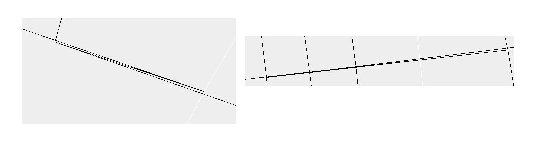
\includegraphics[scale=1.0]{routefailure.eps}
   \caption{Example Failures in Street Map}
   \label{fig:routefailure}
   \end{center}
\end{figure}
\section{Experimental Results}
\label{sec:results}
We repeated the \bmodb{} query execution several times for both data models and
approaches. The tables in Figure \ref{fig:compruntimes} and the graphic in
Figure
\ref{fig:CompTotalRunTimesGraphic} compare the average query run times in
seconds
for the different scale factors, data models, and approaches.
As you can see, the total run time of all queries in NET is around
50\% less than the total query run time of SPACE at each \textit{scalefactor}.
\begin{figure}[h]
  \begin{minipage}{0.5\linewidth}
    \begin{tiny}
      \begin{tabular}{|c|r|r|r|r|}
        \hline
                       & \multicolumn{4}{c|}{\textbf{Scalefactor 0.05}}\\
        \cline{2-5}
                       & \multicolumn{2}{c|}{\textbf{SPACE}} & \multicolumn{2}{c|}{\textbf{NET}}\\
        \hline
        \textbf{Query} & \textbf{OBA} & \textbf{TBA} & \textbf{OBA} & \textbf{TBA}\\
        \hline
        \textbf{1}     &   0.160      &   0.109      &   0.197      &   0.097\\
        \hline
        \textbf{2}     &   0.003      &   0.002      &   0.003      &   0.002\\
        \hline
        \textbf{3}     &   0.418      &   0.279      &   0.462      &   0.595\\
        \hline
        \textbf{4}     &   9.461      &  11.709      &   0.338      &   1.508\\
        \hline
        \textbf{5}     &   1.087      &   1.632      &   1.760      &   1.238\\
        \hline
        \textbf{6}     &  13.391      &   6.461      &   5.933      &   4.016\\
        \hline
        \textbf{7}     &   3.568      &   3.213      &   5.670      &   7.024\\
        \hline
        \textbf{8}     &   0.324      &   0.351      &   0.218      &   0.208\\
        \hline
        \textbf{9}     &  88.124      & 188.896      &  21.618      &  19.758\\
        \hline
        \textbf{10}    & 101.294      &  31.166      &  63.217      &  79.528\\
        \hline
        \textbf{11}    &   0.152      &   0.104      &   1.044      &   1.018\\
        \hline
        \textbf{12}    &   0.285      &   0.109      &   0.203      &   0.177\\
        \hline
        \textbf{13}    &   9.952      &   6.606      &   1.135      &   1.141\\
        \hline
        \textbf{14}    &   0.505      &   0.625      &   1.513      &   3.747\\
        \hline
        \textbf{15}    &   1.036      &   0.783      &   0.599      &   0.501\\
        \hline
        \textbf{16}    &   5.768      &  16.744      &   0.580      &   1.501\\
        \hline
        \textbf{17}    &   1.144      &   1.180      &   0.208      &   0.292\\
        \hline
        \textbf{Total} & 236.670      & 269.970      & 104.698      & 122.352\\
        \hline
      \end{tabular}
    \end{tiny}
  \end{minipage} \hfill
  \begin{minipage}{0.5\linewidth}
    \begin{tiny}
      \begin{tabular}{|c|r|r|r|r|}
        \hline
                       & \multicolumn{4}{c|}{\textbf{Scalefactor 0.2}}\\
        \cline{2-5}
                       & \multicolumn{2}{c|}{\textbf{SPACE}} & \multicolumn{2}{c|}{\textbf{NET}}\\
        \hline
        \textbf{Query} & \textbf{OBA} & \textbf{TBA}  & \textbf{OBA} & \textbf{TBA}\\
        \hline
        \textbf{1}     &    0.122     &    0.101      &    0.166     &    0.113\\
        \hline
        \textbf{2}     &    0.003     &    0.003      &    0.004     &    0.003\\
        \hline
        \textbf{3}     &    0.468     &    0.318      &    0.584     &    0.817\\
        \hline
        \textbf{4}     &   32.742     &   39.531      &    0.604     &    8.663\\
        \hline
        \textbf{5}     &    1.649     &    3.033      &    2.990     &    2.434\\
        \hline
        \textbf{6}     &   66.301     &   48.417      &   17.046     &   14.982\\
        \hline
        \textbf{7}     &   18.444     &   11.435      &   25.204     &   31.675\\
        \hline
        \textbf{8}     &    0.451     &    0.358      &    0.229     &    0.252\\
        \hline
        \textbf{9}     &  246.767     &  373.958      &   33.143     &   44.976\\
        \hline
        \textbf{10}    &  487.731     &  136.743      &  286.764     &  294.473\\
        \hline
        \textbf{11}    &    0.244     &    0.153      &    2.956     &    3.136\\
        \hline
        \textbf{12}    &    4.480     &    0.140      &    0.260     &    0.261\\
        \hline
        \textbf{13}    &   30.072     &   15.216      &    5.314     &    4.646\\
        \hline
        \textbf{14}    &    1.124     &    1.168      &    3.325     &    9.655\\
        \hline
        \textbf{15}    &    8.617     &    4.281      &    2.399     &    1.985\\
        \hline
        \textbf{16}    &    6.967     &   28.592      &    0.365     &    0.824\\
        \hline
        \textbf{17}    &    8.703     &    6.718      &    0.333     &    0.734\\
        \hline
        \textbf{Total} &  914.886     &  670.165      &  381,685     &  419.631\\
        \hline
      \end{tabular}
    \end{tiny}
  \end{minipage}\hfill
\begin{minipage}{0.5\linewidth}
    \begin{tiny}
      \begin{tabular}{|c|r|r|r|r|}
        \hline
        &\multicolumn{4}{c|}{\textbf{Scalefactor 1.0}}\\
        \cline{2-5}
        &\multicolumn{2}{c|}{\textbf{SPACE}}&\multicolumn{2}{c|}{\textbf{NET}}\\
        \hline
        \textbf{Query} & \textbf{OBA} & \textbf{TBA} & \textbf{OBA} & \textbf{TBA}\\
        \hline
        \textbf{1}     &      0.185   &      0.196   &      0.302   &      0.205\\
        \hline
        \textbf{2}     &      0.005   &      0.004   &      0.006   &      0.004\\
        \hline
        \textbf{3}     &      0.948   &      0.540   &      1.207   &      1.418\\
        \hline
        \textbf{4}     &    199.990   &    159.760   &      1.207   &     33.035\\
        \hline
        \textbf{5}     &      3.326   &      6.347   &      5.851   &      5.675\\
        \hline
        \textbf{6}     &   1295.508   &   2099.649   &    300.661   &    235.301\\
        \hline
        \textbf{7}     &    108.222   &     44.631   &    110.542   &    123.349\\
        \hline
        \textbf{8}     &      0.840   &      0.502   &      0.240   &      0.280\\
        \hline
        \textbf{9}     &    795.955   &   1887.512   &    108.343   &    138.995\\
        \hline
        \textbf{10}    &   3564.303   &   2099.858   &   2358.162   &   1661.170\\
        \hline
        \textbf{11}    &      0.737   &      0.650   &      7.804   &      8.702\\
        \hline
        \textbf{12}    &     39.648   &      0.216   &      0.713   &      0.289\\
        \hline
        \textbf{13}    &    118.512   &    78.304    &     27.203   &     34.018\\
        \hline
        \textbf{14}    &     11.494   &     4.990    &      9.423   &     39.700\\
        \hline
        \textbf{15}    &     29.831   &    17.227    &     10.140   &      6.304\\
        \hline
        \textbf{16}    &      9.802   &    60.795    &      0.517   &      1.919\\
        \hline
        \textbf{17}    &     84.209   &   162.730    &      0.554   &      5.829\\
        \hline
        \textbf{Total} &   6263.514   &  6623.912    &   2942.663   &   2295.765\\
        \hline
      \end{tabular}
    \end{tiny}
  \end{minipage}
 \caption{Compare Query Run Times in Seconds}
 \label{fig:compruntimes}
\end{figure}
\begin{figure}
  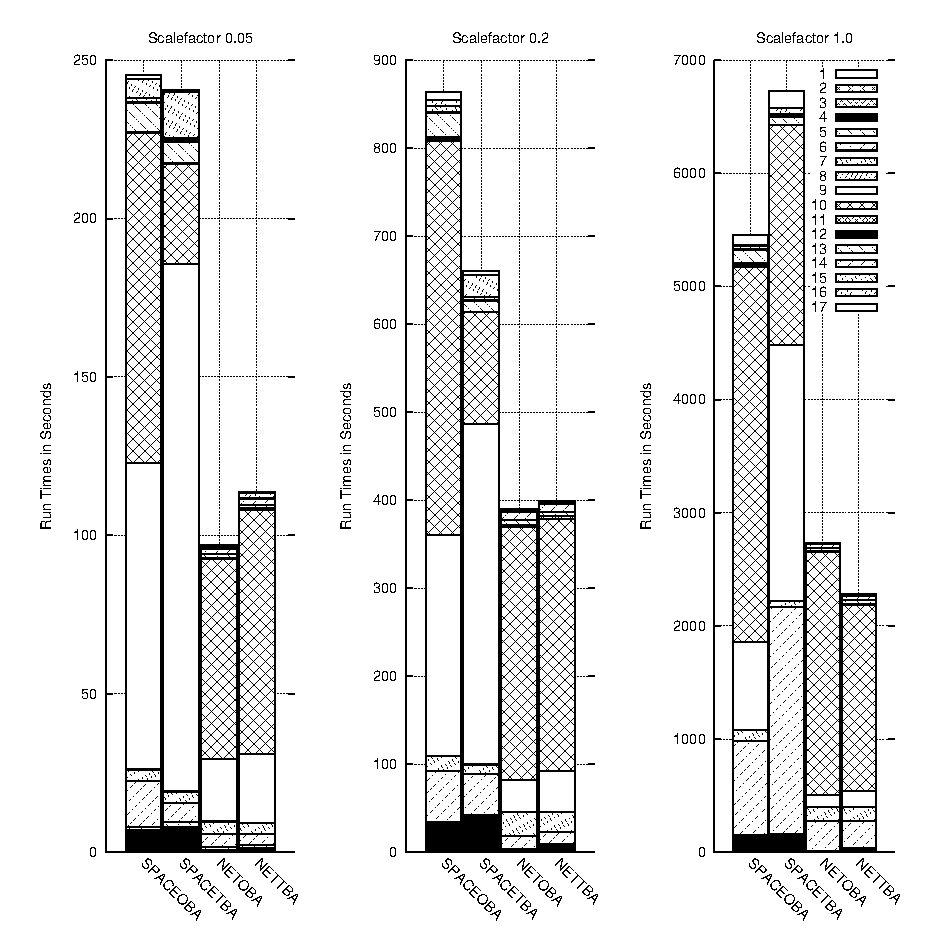
\includegraphics[width=1.0\linewidth]{compruntimesall.eps}
  \caption{Compare Total Run Times}
  \label{fig:CompTotalRunTimesGraphic}
\end{figure}

For the queries 1 and 2, the query run times are almost the same for all data
models
and approaches at the different \textit{scalefactors}. These results are expected,
because
both queries deal only with standard attributes and standard indexes, which
are not influenced by the different data models.

Although the query algorithms for both data models and approaches are almost the
same, SPACE outperforms NET for query 3 by tenths of a second. On the one hand,
the
number of units in NET is less than the number of units in SPACE,
such that the unit which contains the query time instant should be found faster.
But on the other hand, a \dt{gpoint} value has more internal elements (3
\dt{int},
1 \dt{real}, and 1 \dt{bool}) than a \dt{point} value (2 \dt{real}, and 1
\dt{bool}),
such that each unit in NET has more elements than in SPACE, therefore
access and copying needs a little more time in NET than in SPACE.

In query 4 NET outperforms SPACE significantly at all \textit{scalefactors} ($>$ 3 min
OBA,
$>$ 2 min TBA at \textit{scalefactor} 1.0). The NET index used in query 4 is
much smaller
(OBA 24 MB, TBA 160 MB, at \textit{scalefactor} 1.0) than the spatial unit index
of SPACE
(OBA 3.7 GB, TBA 3.7 GB at \textit{scalefactor} 1.0) and more precise, such that
we do not
need an additional expensive refinement step after the index usage in NET,
like we do in SPACE.

We expected NET to be slower than SPACE in the queries 5, 6, and 10, because
we retranslate intermediate results from NET representation into SPACE
representation.
For query 5 this holds in the OBA. We need a little more time in NET
than in SPACE. But in TBA NET outperforms SPACE. This is due to the fact
that a \dt{gline} value has less \textit{route intervals}
than a \dt{line} value has line segments,
such that the union of \dt{gline} values in the aggregate step of query 5 in
TBA can be computed much faster in NET than the union of \dt{line} values in SPACE.

NET outperforms SPACE again significantly at query 6
for all amounts of data and approaches ($>$ 15 minutes for OBA, $>$
30 minutes for TBA, at \textit{scalefactor} 1.0). In NET we reduce the number of
candidate
pairs for the distance computation by some filter steps, while in SPACE
in the OBA no filtering is used. NET uses the operation \op{everNearerThan}, which
stops computation immediately if the distance between two units is less than the
query value. Whereas the operation \op{distance} used by SPACE in OBA always checks
all units of the query objects. For the TBA SPACE uses \op{everNearerThan}
instead of \op{distance} and a filter step before. But, whereas NET uses in TBA
a spatio-temporal filtering, SPACE uses only a spatial filtering, such that many
false candidates are included in the expensive distance computation part of the
algorithm.

After the very good results from query 4 we did not expect SPACE to outperform
NET at query 7. The weakness of NET is that we have to do the expensive \op{at} 
operation for the double number of query \dt{gpoint} compared with SPACE
(see Section \ref{sec:translateSTdata}).
But in the end, NET looses at \textit{scalefactor} 1.0 around 2 seconds in OBA
and 80 seconds in TBA, what is not much compared with the advantages in the other
benchmark queries.

Query 8 is a very fast query in both data models, although the query run time of
NET is more than 30\% less than the query run time of SPACE. This is caused by the
\textit{length} attribute of the \dt{mgpoint} and the smaller number of units of a
\dt{mgpoint} compared with the corresponding \dt{mpoint}.

For query 9, NET outperforms SPACE by orders of magnitude. The advantages
named in the analysis of query 8 have a much more impact
when the number of examined trips becomes higher. At \textit{scalefactor} 1.0
this saves
more than 10 minutes time in the OBA and more than 25 minutes time in the TBA.

The ratio of the run times of query 10 changes between the amounts of data and
both data models. In the OBA NET outperforms SPACE at all \textit{scalefactors}
and at \textit{scalefactor} 1.0 in TBA, whereas SPACE outperforms NET for the
lower amounts of data in TBA significantly.
Before our experiments we expected that SPACE would outperform NET in all cases,
because of the expensive retranslation of intermediate results.
So why is NET 20 minutes faster at \textit{scalefactor} 1.0 in OBA than SPACE?
In NET we use bounding boxes to preselect candidate trips that step is not
performed in SPACE. The disadvantage of NET in TBA becomes smaller at higher
\textit{scalefactors} we think this is due to the fact that the number of units in
\dt{mgpoint} values is always smaller than in \dt{mpoint} values such that the
final aggregation of the different trips of the same cars can be done faster
in NET than SPACE.

In our experiments we also tested the MON-Tree \cite{MONTreeAlmeidaGeoinformatica}
as spatio-temporal index. But, although the CPU run time was very small, the
elapsed run time performance was very bad. Such that the primitive index outperformed
the MON-Tree in all cases.

Query 11 is identical with the first part of query 12. So it is surprising that
the run time of query 11 is longer than the run time of query 12,
which does additional computations. In our experiments with the different queries
we have seen that there exist numerous cache effects depending on the sequence of
the queries. So we think that query 12 takes profit of cache effects resulting from
query 11 running immediately before query 12. Another weakness of NET pointed
out by the run times of query 11 and some other queries is that our TNPI has bad
run times for query TNBB created from a single \dt{gpoint} and a single
time instant. This becomes worse with a higher number of indexed units. As you can
see at query 15 this does not hold for query TNBB constructed from a single
\dt{gpoint} and a time interval. We have to spend some more work to figure out
the problem and develop a better TNPI to improve our NET implementation.

The bad performance of the TNPI is also shown by query 13.
NET outperforms SPACE significantly, but we do not use any index in the
executable NET queries, while SPACE uses its spatio-temporal index to preselect
candidate trips. The same holds for query 17.

The NET version of query 16 takes profit from the smaller number
of units in NET and outperforms SPACE significantly.

Although we detected in our experiments some points of weakness in the temporal 
network position index (TNPI), NET outperforms SPACE by orders of magnitude. The 
weakness of NET almost occurs in queries with short run times, whereas the advantages
of NET become apparent in the queries with long run times, such that the weakness
of the TNPI in some cases is covered by the advantages of NET in the other cases.
\section{Summary and Future Work}
\label{sec:summary}
We presented our translation of the \bmodb{} into the network constrained data model
NET and compared the capabilities of both data models, with very good results for 
NET. Our experiments show that NET outperforms
SPACE by orders of magnitude with respect to storage space and query run times.
This is mainly caused by the much lower number of units for an \dt{mgpoint} value
compared with the number of units of the corresponding \dt{mpoint}, which also
results in smaller indexes for NET objects. The \bmodb{} of NET pointed out
that we should spend time in the improvement of the TNPI.

The good results of NET encourages to spend further work in the network representation 
of network constrained objects. 

We want to extend the \bmodb{}, with an additional query set, covering the 
special challenges of spatio-temporal network constrained databases like
shortest path computing. The new query set should enable us to compare the
capabilites of database systems dealing with spatio-temporal NCDM.

Another direction of our actual work is traffic flow estimation and traffic jam
representation in NET.

An interesting topic for future work on NCDM is the efficient
computation of dynamic network distances between moving objects in the network.
\bibliography{BerlinMODAndNetworkDataModel}{}
\bibliographystyle{plain}
\appendix
\section{Executable \secondo{} NET Queries}
\label{app:executableQueries}
In the sequel we present our executable \secondo{} queries for the NET representation
of the \bmodb{}. The name of the query result object indicates the number of
the query, and if it is a query for the object based approach (OBA), or for the
trip based approach (TBA).
\begin{scriptsize}
\begin{tabbing}
xxx\=xxx\=xxx\=xxx\=xxx\=xxx\=xxx\=xxx\=xxx\=xxxxxxxxxxxxxxxxxxxxxxxxxxxxxx\kill
\op{let} Q1OBA =\\
\>QueryLicences \op{feed} \{l\}\\
\>\op{loopjoin} [dataSNcar\_Licence\_btree dataSNcar \op{exactmatch} [.Licence\_l]]\\
\>\op{project} [Licence, Model]\\
\op{consume};\\
\\
\op{let} Q1TBA =\\
\>QueryLicences \op{feed} \{l\}\\
\>\op{loopjoin} [dataMcar\_Licence\_btree dataMcar \op{exactmatch} [.Licence\_l]]\\
\>\op{project} [Licence, Model]\\
\op{consume};\\
\\
\op{let} Q2OBA = dataSNcar \op{feed filter} [.Type = 'passenger'] \op{count};\\
\\
\op{let} Q2TBA = dataMcar \op{feed filter} [.Type = 'passenger'] \op{count};\\
\\
\op{let} Q3OBA =\\
\>QueryLicences1 \op{feed} \{l\}\\
\>\>\op{loopjoin} [dataSNcar\_Licence\_btree dataSNcar \op{exactmatch} [.Licence\_l]]\\
\>\>\op{project} [Licence, Trip]\\
\>QueryInstant1 \op{feed} \{i\}\\
\>\op{product}\\
\>\op{projectextend}[Licence, Instant\_i; Pos: \op{val}(.Trip \op{atinstant} .Instant\_i)]\\
\op{consume};\\
\\
\op{let} Q3TBA =\\
\>QueryLicences1 \op{feed} \{l\}\\
\>\>\op{loopsel} [dataMcar\_Licence\_btree dataMcar \op{exactmatch} [.Licence\_l] \{ll\}]\\
\>\>\op{loopjoin} [dataMNtrip\_Moid\_btree dataMNtrip
\op{exactmatch} [.Moid\_ll]]\\
\>QueryInstant1 \op{feed} \{i\}\\
\>\op{symmjoin} [.Trip \op{present} ..Instant\_i]\\
\>\op{projectextend} [Instant\_i, Licence\_ll; Pos: \op{val}(.Trip
\op{atinstant} .Instant\_i)]\\
\op{consume};\\
\\
\op{let} Q4OBA =\\
\> QueryPointsNet \op{feed projectextend} [Id, Pos; Prect: \op{gpoint2rect}(.Pos)]\\
\>\op{loopjoin}[dataSNcar\_TrajBoxNet \op{windowintersectsS} [.Prect]\\
\>\>\>\op{sort rdup} dataSNcar \op{gettuples}]\\
\>\op{project} [Id, Licence]\\
\>\op{sortby} [Id \op{asc}, Licence \op{asc}]\\
\>\op{krdup} [Id, Licence]\\
\op{consume};\\
\\
\op{let}Q4TBA =\\
\>QueryPointsNet \op{feed projectextend} [Id; Elem: \op{gpoint2rect}(.Pos)]\\
\>\op{loopjoin}[dataMNtrip\_TrajBoxNet \op{windowintersectsS} [.Elem]\\
\>\>\>\op{sort rdup} dataMNtrip \op{gettuples}]\\
\>\op{project} [Moid, Id]\\
\>\op{loopsel}[\op{fun}(t:TUPLE) dataMcar\_Moid\_btree dataMcar \op{exactmatch} [\op{attr}(t, Moid)]\\
\>\>\op{projectextend} [Licence; Id: \op{attr}(t, Id)]]\\
\>\op{sortby} [Id \op{asc}, Licence \op{asc}]\\
\>\op{krdup} [Id, Licence]\\
\op{consume};\\
\\
\op{let} Q5h1OBA =\\
\>QueryLicences1 \op{feed} \{l1\}\\
\>\op{loopsel} [dataSNcar\_Licence\_btree dataSNcar \op{exactmatch} [.Licence\_l1]\\
\>\>\op{projectextend} [Licence; TrajLine: \op{gline2line}(\op{trajectory}(.Trip))]]\\
\op{consume};\\
\op{let} Q5h2OBA =\\
\>QueryLicences2 \op{feed} \{l2\}\\
\>\op{loopsel} [dataSNcar\_Licence\_btree dataSNcar \op{exactmatch} [.Licence\_l2]\\
\>\>\op{projectextend} [Licence; TrajLine: \op{gline2line}(\op{trajectory}(.Trip))]]\\
\op{consume};\\
\op{let} Q5OBA =\\
\>Q5h1OBA \op{feed} \{c1\}\\
\>Q5h2OBA \op{feed} \{c2\}\\
\>\op{product}
\>\op{projectextend} [Licence\_c1, Licence\_c2; Distance: \op{distance}(.TrajLine\_c1, .TrajLine\_c2)]\\
\op{consume};\\
\op{delete} Q5h1OBA;\\
\op{delete} Q5h2OBA;\\
\\
\op{let} Q5TBA =\\
\>QueryLicences1 \op{feed project} [Licence] \{LL1\}\\
\>\>\op{loopsel} [\op{fun} (t:TUPLE) dataMcar\_Licence\_btree dataMcar \op{exactmatch} [\op{attr}(t, Licence\_LL1)] \{CAR\}\\
\>\>\>\op{loopsel} [dataMNtrip\_Moid\_btree dataMNtrip \op{exactmatch} [.Moid\_CAR]]\\
\>\>\>\op{projectextend}  [; Traj: \op{trajectory}(.Trip)]\\
\>\>\>\op{aggregateB} [Traj; \op{fun} (L1: gline, L2: gline) L1 \op{union} L2; [\op{const} gline value ()]]\\
\>\>\>\op{feed namedtransformstream} [Traxj]\\
\>\>\>\op{extend} [Licence: \op{attr}(t, Licence\_LL1)]]\\
\>\>\op{projectextend} [Licence; Trax: \op{gline2line}(.Traxj)]\{c1\}\\
\>QueryLicences2 \op{feed} \op{project} [Licence] \{LL2\}\\
\>\>\op{loopsel} [\op{fun} (s:TUPLE) dataMcar\_Licence\_btree dataMcar \op{exactmatch} [\op{attr}(s, Licence\_LL2)] \{CAR\}\\
\>\>\>\op{loopsel} [dataMNtrip\_Moid\_btree dataMNtrip \op{exactmatch} [.Moid\_CAR]]\\
\>\>\>\op{projectextend} [; Traj: \op{trajectory}(.Trip)]\\
\>\>\>\op{aggregateB} [Traj; \op{fun} (L3: gline, L4: gline) L3 \op{union} L4; [\op{const} gline value ()]]\\
\>\>\>\op{feed namedtransformstream} [Traxj]\\
\>\>\>\op{extend} [Licence: \op{attr}(s, Licence\_LL2)]]\\
\>\>\op{projectextend} [Licence; Trax: \op{gline2line}(.Traxj)] \{c2\}\\
\>\op{product}\\
\>\op{projectextend}[Licence\_c1, Licence\_c2; Distance: \op{distance}(.Trax\_c1, .Trax\_c2)]\\
\op{consume};\\
\\
\op{let} Q6hOBA =\\
\>dataSNcar \op{feed filter} [.Type = 'truck']\\
\>\op{projectextend} [Licence; ptrip: \op{mgpoint2mpoint}(.Trip), BBox: \op{mgpbbox}(.Trip)]\\
\>\op{projectextend} [Licence, ptrip; Box: \op{rectangle3}(\op{minD}(.BBox, 1) - 5.0, \op{maxD}(.BBox, 1) + 5.0,\\
\>\>\>\>\op{minD}(.BBox, 2) - 5.0, \op{maxD}(.BBox, 2) + 5.0, \op{minD}(.BBox, 3), \op{maxD}(.BBox, 3))]\\
\op{consume};\\
\op{let} Q6OBA =\\
\>Q6hOBA \op{feed} \{a\}\\
\>Q6hOBA \op{feed} \{b\}\\
\>\op{symmjoin}[(.Box\_a \op{intersects} ..Box\_b) \op{and} (.Licence\_a $<$ ..Licence\_b) \op{and}\\
\>\>\>\>(\op{everNearerThan}(.ptrip\_a, ..ptrip\_b, 10.0))]\\
\>\op{project} [Licence\_a, Licence\_b]\\
\>\op{sortby} [Licence\_a \op{asc}, Licence\_b \op{asc}]\\
\>\op{krdup} [Licence\_a, Licence\_b]\\
\op{consume};\\
\op{delete} Q6hOBA;\\
\\
\op{let} Q6hTBA =\\
\>dataMcar \op{feed filter} [.Type = 'truck'] \op{project} [Licence, Moid] \{c\}\\
\>\op{loopjoin} [dataMNtrip\_Moid\_btree dataMNtrip \op{exactmatch} [.Moid\_c]]\\
\>\op{projectextend} [; Licence: .Licence\_c, BBox: \op{mgpbbox}(.Trip), ptrip: \op{mgpoint2mpoint}(.Trip)]\\
\>\op{projectextend} [Licence, ptrip; Box: \op{rectangle3}((\op{minD}(.BBox, 1) - 5.0), (\op{maxD}(.BBox, 1) + 5.0),\\
\>\>\>\>(\op{minD}(.BBox, 2) - 5.0), (\op{maxD}(.BBox, 2) + 5.0), \op{minD}(.BBox, 3), \op{maxD}(.BBox, 3))]\\
\op{consume};\\
\op{let} Q6TBA =\\
\>Q6hTBA \op{feed} \{c1\}\\
\>Q6hTBA \op{feed} \{c2\}\\
\>\op{symmjoin} [(.Box\_c1 \op{intersects} ..Box\_c2) \op{and} (.Licence\_c1 $<$ ..Licence\_c2)]\\
\>\op{filter} [\op{everNearerThan}(.ptrip\_c1, .ptrip\_c2, 10.0)]\\
\>\op{project} [Licence\_c1, Licence\_c2]\\
\>\op{sortby} [Licence\_c1 \op{asc}, Licence\_c2 \op{asc}]\\
\>\op{krdup} [Licence\_c1, Licence\_c2]\\
\op{consume};\\
\op{delete} Q6hTBA;\\
\\
\\op{let} Q7hOBA =\\
\>QueryPointsNet \op{feed projectextend} [Id, Pos; Prect: \op{gpoint2rect}(.Pos)]\\
\>\op{loopsel} [\op{fun} (t:TUPLE) dataSNcar\_TrajBoxNet \op{windowintersectsS}[\op{attr}(t, Prect)]\\
\>\>\op{sort rdup} dataSNcar \op{gettuples}\\
\>\>\op{filter} [.Type = 'passenger']\\
\>\>\op{projectextend} [Licence; Id: \op{attr}(t, Id), Instant: \op{inst}(\op{initial}(.Trip \op{at attr}(t, Pos)))]]\\
\>\op{filter} [\op{not}(\op{isempty}(.Instant))]\\
\>\op{sortby} [Id \op{asc}, Instant \op{asc}]\\
\op{consume};\\
\op{let} Q7cOBA =\\
\>Q7hOBA \op{feed groupby} [Id; FirstTime: \op{group feed min} [Instant]] \{b\}\\
\>Q7hOBA \op{feed} \{a\}\\
\>\op{symmjoin} [..Id\_a = .Id\_b]\\
\>\op{filter} [.Instant\_a $\leq$ .FirstTime\_b]\\
\>\op{project} [Id\_a, Licence\_a]\\
\op{consume};\\
\op{delete} Q7hOBA;\\
\\
\op{let} Q7hTBA =\\
\>QueryPointsNet \op{feed projectextend} [Id, Pos; Prect: \op{gpoint2rect}(.Pos)]\\
\>\op{loopsel} [\op{fun} (t:TUPLE) dataMNtrip\_TrajBoxNet \op{windowintersectsS} [\op{attr} (t, Prect)]\\
\>\>\op{sort rdup} dataMNtrip \op{gettuples}\\
\>\>\op{loopjoin} [dataMcar\_Moid\_btree dataMcar exactmatch [.Moid]\\
\>\>\>\op{filter} [.Type = 'passenger']\\
\>\>\>\op{project} [Licence] \{X\}]\\
\>\>\op{projectextend} [Licence\_X; TimeAtPos: \op{inst}(\op{initial}(.Trip \op{at attr}(t, Pos))), Id: \op{attr}(t, Id)]]\\
\>\op{sortby} [Id \op{asc}, TimeAtPos \op{asc}]\\
\op{consume};\\
\op{let} Q7aTBA =\\
\>Q7hTBA \op{feed groupby} [Id; FirstTime: \op{group feed min} [TimeAtPos]] \{b\}\\
\>Q7hTBA \op{feed} \{a\}\\
\>\op{symmjoin} [..Id\_a = .Id\_b]\\
\>\op{filter} [.TimeAtPos\_a $\leq$ .FirstTime\_b]\\
\>\op{project} [Id\_a, Licence\_X\_a]\\
\>\op{sortby} [Id\_a \op{asc}, Licence\_X\_a \op{asc}]\\
\>\op{krdup} [Id\_a, Licence\_X\_a]\\
\op{consume};\\
\op{delete} Q7hTBA;\\
\\
\op{let} Q8OBA =\\
\>QueryLicences1 \op{feed} \{l\}\\
\>\>\op{loopsel} [dataSNcar\_Licence\_btree dataSNcar \op{exactmatch}
[.Licence\_l]]\\
\>QueryPeriods1 \op{feed filter}[\op{not}(\op{isempty}(.Period))] \{p\}\\
\>\op{product}\\
\>\op{projectextend} [Licence, Period\_p; Distance: \op{length}(.Trip
\op{atperiods} .Period\_p)]\\
\op{consume};\\
\\
\op{let} Q8TBA =\\
\>QueryLicences1 \op{feed} \{l\}\\
\>\>\op{loopjoin} [dataMcar\_Licence\_btree dataMcar \op{exactmatch} [.Licence\_l]]\\
\>\>\op{project} [Licence, Moid]\\
\>\>\op{loopsel} [\op{fun} (t:TUPLE) dataMNtrip\_Moid\_btree dataMNtrip \op{exactmatch} [\op{attr}(t, Moid)]\\
\>\>\>\op{projectextend}[Trip; Licence: \op{attr}(t, Licence)]]\\
\>QueryPeriods1 \op{feed}\\
\>\op{symmjoin} [.Trip \op{present} ..Period]\\
\>\op{projectextend} [Licence, Period, Id; Distance: \op{length}(.Trip \op{atperiods} .Period)]\\
\>\op{sortby} [Id \op{asc}, Licence \op{asc}, Distance \op{desc}]\\
\>\op{groupby} [Id, Period, Licence; Dist: \op{group feed sum} [Distance]]\\
\>\op{project} [Licence, Period, Dist]\\
\op{consume};\\
\\
\op{let} Q9OBA =\\
\>dataSNcar \op{feed} \{c\}\\
\>QueryPeriods \op{feed filter} [\op{not}(\op{isempty}(.Period))] \{p\}\\
\>\op{product}\\
\>\op{projectextend} [Id\_p, Period\_p, Licence\_c; Dist: \op{length}(.Trip\_c \op{atperiods} .Period\_p)]\\
\>\op{sortby} [Id\_p \op{asc}, Period\_p \op{asc}, Dist \op{desc}]\\
\>\op{groupby} [Id\_p, Period\_p; Distance: \op{group feed max} [Dist]]\\
\>\op{project} [Id\_p, Period\_p, Distance]\\
\>\op{sortby} [Id\_p \op{asc}]\\
\>\op{project} [Period\_p, Distance]\\
\op{consume};\\
\\
\op{let} Q9TBA =\\
\>dataMNtrip \op{feed} \{c\}\\
\>QueryPeriods \op{feed filter} [\op{not}(\op{isempty}(.Period))] \{p\}\\
\>\op{symmjoin}[.Trip\_c \op{present} ..Period\_p]\\
\>\op{projectextend} [Moid\_c, Period\_p, Id\_p; Distance: \op{length}(.Trip\_c \op{atperiods} .Period\_p)]\\
\>\op{sortby} [Id\_p \op{asc}, Moid\_c \op{asc}, Distance \op{desc}]\\
\>\op{groupby} [Id\_p, Period\_p, Moid\_c; Dist: \op{group feed sum} [Distance]]\\
\>\op{groupby} [Id\_p, Period\_p; Dista: \op{group feed max} [Dist]]\\
\>\op{project} [Period\_p, Dista]\\
\op{consume};\\
\\
\op{let} Q10OBA =\\
\>dataSNcar \op{feed}\\
\>\>\op{projectextend}[Licence; TripA: \op{mgpoint2mpoint}(.Trip), BBox: \op{mgpbbox}(.Trip)]\\
\>\>\op{projectextend}[Licence, TripA; Box: \op{rectangle2}((\op{minD}(.BBox, 1) - 1.5), (\op{maxD}(.BBox, 1) + 1.5),\\
\>\>\>\>(\op{minD}(.BBox, 2) - 1.5), (\op{maxD}(.BBox, 2) + 1.5))] \{c1\}\\
\>QueryLicences1 \op{feed}\\
\>\>\op{loopsel} [dataSNcar\_Licence\_btree dataSNcar \op{exactmatch} [.Licence]]\\
\>\>\op{projectextend} [Licence, Trip;  BBox: \op{mgpbbox}(.Trip)]\\
\>\>\op{projectextend} [Licence, Trip; TripA: \op{mgpoint2mpoint}(.Trip), Box: \op{rectangle2}(\op{minD}(.BBox,1) - 1.5),\\
\>\>\>\>(\op{maxD}(.BBox, 1) + 1.5), (\op{minD}(.BBox, 2) - 1.5), (\op{maxD}(.BBox, 2) + 1.5))] \{c2\}\\
\>\op{symmjoin} [.Box\_c1 \op{intersects} ..Box\_c2]\\
\>\op{filter} [.Licence\_c1 $\neq$ .Licence\_c2]\\
\>\op{filter} [\op{everNearerThan}(.TripA\_c1, .TripA\_c2, 3.0)]\\
\>\op{projectextend} [Licence\_c1, Licence\_c2; \\
\>\>\>\>Pos: .Trip\_c2 \op{atperiods deftime}((\op{distance}(.TripA\_c1, .TripA\_c2) $<$ 3.0) \op{at} \true{}]\\
\>\op{filter} [\op{not}(\op{isempty}(.Pos))]\\
\>\op{project} [Licence\_c2, Licence\_c1, Pos]\\
\>\op{sortby} [Licence\_c2 \op{asc}, Licence\_c1 \op{asc}]\\
\op{consume};\\
\\
\op{let} Q10TBA =\\
\>QueryLicences1 \op{feed project} [Licence] \{V1\}\\
\>\op{loopsel} [\op{fun} (t:TUPLE) dataMcar\_Licence\_btree dataMcar \op{exactmatch} [\op{attr}(t, Licence\_V1)]\\
\>\>\op{project} [Moid]\\
\>\>\op{loopjoin} [dataMNtrip\_Moid\_btree dataMNtrip \op{exactmatch} [.Moid] \op{remove}[Moid]] \{V3\}\\
\>\>\op{extend} [t3bbx: \op{mgpbbox}(.Trip\_V3)]\\
\>\>\op{extend} [ptripA: \op{mgpoint2mpoint}(.Trip\_V3)]\\
\>\>\op{loopjoin} [\op{fun} (u:TUPLE) dataMNtrip\_SpatioTemp \op{windowintersectsS}[\op{rectangle3}(\\
\>\>\>\>\op{minD}(\op{attr}(u, t3bbx), 1) - 3.0, \op{maxD}(\op{attr}(u, t3bbx), 1) + 3.0,\\
\>\>\>\>\op{minD}(\op{attr}(u, t3bbx), 2) - 3.0, \op{maxD}(\op{attr}(u, t3bbx), 2) + 3.0,\\
\>\>\>\>\op{minD}(\op{attr}(u, t3bbx), 3), \op{maxD}(\op{attr}(u, t3bbx), 3))]\\
\>\>\>\op{sort rdup} dataMNtrip \op{gettuples}\\
\>\>\>\op{filter} [.Moid $\neq$ \op{attr}(u, Moid\_V3)]\\
\>\>\>\op{projectextend} [Moid; ptripB: \op{mgpoint2mpoint}(.Trip)]\\
\>\>\>\op{filter} [\op{everNearerThan}(\op{attr}(u, ptripA), .ptripB, 3.0)]\\
\>\>\>\op{projectextend} [Moid; Times: \op{deftime}((\op{distance}(\op{attr}(u, ptripA), .ptripB) $<$ 3.0) \op{at} \true{})]\\
\>\>\>\op{filter} [\op{not}(\op{isempty}(.Times))]\\
\>\>\>\op{loopjoin} [dataMcar\_Moid\_btree dataMcar \op{exactmatch} [.Moid] \op{project} [Licence]]]\\
\>\>\op{projectextend} [Times, Trip\_V3; QueryLicence: \op{attr}(t, Licence\_V1), OtherLicence: .Licence]\\
\>\>\op{projectextend} [QueryLicence, OtherLicence; Pos: .Trip\_V3 \op{atperiods} .Times]\\
\>\>\op{filter} [\op{not}(\op{isempty}(.Pos))]]\\
\>\op{sortby} [QueryLicence \op{asc}, OtherLicence \op{asc}]\\
\>\op{groupby} [QueryLicence, OtherLicence; AllPos: \op{group feed aggregateB}[Pos;\\
\>\>\>\op{fun} (M1:mgpoint, M2:mgpoint) M1 \op{union} M2; [\op{const} mgpoint value()]]]\\
\>\op{project} [QueryLicence, OtherLicence, AllPos]\\
\op{consume};\\
\\
\op{let} Q11bOBA =\\
\>QueryInstant1 \op{feed} \{i\}\\
\>QueryPoints1Net \op{feed projectextend} [Id, Pos; Prect: \op{gpoint2rect}(.Pos)] \{p\}\\
\>\op{product}\\
\>\op{projectextend} [Id\_p, Instant\_i; Box: \op{box3d}(.Prect\_p, .Instant\_i)]\\
\>\op{loopsel} [\op{fun}(t:TUPLE) dataSNcar\_BoxNet\_timespace \op{windowintersectsS} [\op{attr}(t, Box)]\\
\>\>\op{sort rdup} dataSNcar \op{gettuples}\\
\>\>\op{projectextend} [Licence; Id: \op{attr}(t, Id\_p), Instant\_i: \op{attr}(t, Instant\_i)]]\\
\op{consume};\\
\\
\op{let} Q11TBA =\\
\>QueryInstant1 \op{feed} \{i\}\\
\>QueryPoints1Net \op{feed projectextend} [Id, Pos; Prect: \op{gpoint2rect}(.Pos)] \{p\}\\
\>\op{product}\\
\>\op{loopsel} [\op{fun} (t:TUPLE) dataMNtrip\_BoxNet\_timespace \op{windowintersectsS}[\\ 
\>\>\>\op{box3d}(\op{attr}(t, Prect\_p), \op{attr}(t, Instant\_i))]\\
\>\>\op{sort rdup} dataMNtrip \op{gettuples}\\
\>\>\op{projectextend} [Moid; Id: \op{attr}(t, Id\_p), Instant: \op{attr}(t, Instant\_i)]] \{a\}\\
\>\op{loopjoin} [dataMcar\_Moid\_btree dataMcar \op{exactmatch} [.Moid\_a]]\\
\>\op{project} [Id\_a, Instant\_a, Licence]\\
\>\op{sortby} [Id\_a \op{asc}, Instant\_a \op{asc}, Licence \op{asc}]\\
\>\op{krdup} [Id\_a, Instant\_a, Licence]\\
\op{consume};\\
\\
\op{let} Q12hOBA =\\
\>QueryInstant1 \op{feed} \{i\}\\
\>QueryPoints1Net \op{feed projectextend} [Id, Pos; Prect: \op{gpoint2rect}(.Pos)] \{p\}\\
\>\op{product}\\
\>\op{loopsel} [\op{fun} (t:TUPLE) dataSNcar\_BoxNet\_timespace windowintersectsS[\\
\>\>\>\op{box3d}(\op{attr}(t, Prect\_p), \op{attr}(t, Instant\_i))]\\
\>\>\op{sort rdup} dataSNcar \op{gettuples}\\
\>\>\op{projectextend} [Licence; Id\_p: \op{attr}(t, Id\_p), Pos\_p: \op{attr}(t, Pos\_p), Instant\_i: \op{attr}(t, Instant\_i)]]\\
\>\op{sortby} [Id\_p \op{asc}, Instant\_i \op{asc}, Licence \op{asc}]\\
\op{consume};\\
\op{let} Q12OBA =\\
\>Q12hOBA \op{feed} \{c1\}\\
\>Q12hOBA \op{feed} \{c2\}\\
\>\op{symmjoin} [(.Licence\_c1 $<$ ..Licence\_c2) \op{and} (.Id\_p\_c1 = ..Id\_p\_c2) \op{and} (.Instant\_i\_c1 = ..Instant\_i\_c2)]\\
\>\op{project} [Id\_p\_c1, Pos\_p\_c1, Instant\_i\_c1, Licence\_c1, Licence\_c2]\\
\>\op{sortby} [Id\_p\_c1 \op{asc}, Instant\_i\_c1 \op{asc}, Licence\_c2 \op{asc}]\\
\op{consume};\\
\op{delete} Q12hOBA;\\
\\
\op{let} Q12hTBA =\\
\>QueryPoints1Net \op{feed projectextend} [Id, Pos; Prect: \op{gpoint2rect}(.Pos)] \{p\}\\
\>QueryInstant1 \op{feed} \{i\}\\
\>\op{product}\\
\>\op{projectextend} [Id\_p, Pos\_p, Instant\_i; Box: \op{box3d}(.Prect\_p, .Instant\_i)]\\
\>\op{loopsel} [\op{fun} (t:TUPLE) dataMNtrip\_BoxNet\_timespace \op{windowintersectsS} [\op{attr}(t, Box)]\\
\>\>\op{sort rdup} dataMNtrip \op{gettuples}\\
\>\>\op{projectextend} [Moid; Id: \op{attr}(t, Id\_p), Instant: \op{attr}(t, Instant\_i)]] \{a\}\\
\>\op{loopjoin} [dataMcar\_Moid\_btree dataMcar \op{exactmatch} [.Moid\_a]]\\
\>\op{projectextend} [Moid, Licence; Id: .Id\_a, Instant: .Instant\_a]\\
\op{consume};\\
\op{let} Q12TBA =\\
\>Q12hTBA \op{feed} \{A\}\\
\>Q12hTBA \op{feed} \{B\}\\
\>\op{symmjoin} [(.Id\_A = ..Id\_B) \op{and} (.Instant\_A = ..Instant\_B) \op{and} (.Moid\_A $<$ ..Moid\_B)]\\
\>\op{project} [Id\_A, Instant\_A, Licence\_A, Licence\_B]\\
\>\op{sortby} [Id\_A \op{asc}, Instant\_A \op{asc}, Licence\_B \op{asc}]\\
\op{consume};\\
\op{delete} Q12hTBA;\\
\\
\op{let} Q13OBA =\\
\>dataSNcar \op{feed} \{c\}\\
\>QueryRegions1Net \op{feed filter} [\op{not}(\op{isempty}(.Region))] \{r\}\\
\>\op{symmjoin} [.Trip\_c \op{passes} ..Region\_r]\\
\>\>\op{projectextend} [Licence\_c, Id\_r, Region\_r; Trip: .Trip\_c \op{at} .Region\_r]\\
\>QueryPeriods1 \op{feed filter} [\op{not}(\op{isempty}(.Period))] \{p\}\\
\>\op{symmjoin} [.Trip \op{present} ..Period\_p]\\
\>\op{projectextend} [Id\_r, Period\_p; Licence: .Licence\_c, Trip: .Trip \op{atperiods} .Period\_p]\\
\>\op{filter} [\op{no\_components}(.Trip) $>$ 0]\\
\>\op{project} [Id\_r, Period\_p, Licence]\\
\>\op{sortby} [Id\_r \op{asc}, Period\_p \op{asc}, Licence \op{asc}]\\
\op{consume};\\
\\
\op{let} Q13TBA =\\
\>dataMNtrip \op{feed} \{c\}\\
\>QueryRegions1Net \op{feed filter} [\op{not}(\op{isempty}(.Region))] \{r\}\\
\>\op{symmjoin} [.Trip\_c \op{passes} ..Region\_r]\\
\>\>\op{projectextend} [Moid\_c, Id\_r; Trip: .Trip\_c \op{at} .Region\_r]\\
\>QueryPeriods1 \op{feed filter} [\op{not}(\op{isempty}(.Period))] \{p\}\\
\>\op{symmjoin} [.Trip \op{present} ..Period\_p]\\
\>\op{loopjoin} [dataMcar\_Moid\_btree dataMcar \op{exactmatch} [.Moid\_c]]\\
\>\op{project} [Licence, Id\_r, Period\_p]\\
\>\op{sortby} [Id\_r \op{asc}, Period\_p \op{asc}, Licence \op{asc}]\\
\>\op{krdup} [Id\_r, Period\_p, Licence]\\
\op{consume};\\
\\
\op{let} Q14aOBA =\\
\>dataSNcar \op{feed}\\
\>QueryInstant1 \op{feed}\\
\>\op{product}\\
\>\>\op{projectextend} [Licence, Instant; PosX: \op{val}(.Trip \op{atinstant} .Instant)]\\
\>\>\op{projectextendstream} [Licence, Instant; Pos: polygpoints(.PosX, B\_NETWORK)]\\
\>QueryRegions1Net \op{feed filter} [\op{not}(\op{isempty}(.Region))]\\
\>\op{symmjoin} [.Pos \op{inside} ..Region]\\
\>\op{project} [Id, Instant, Licence]\\
\>\op{sortby} [Id \op{asc}, Instant \op{asc}, Licence \op{asc}]\\
\>\op{krdup}[Id, Instant, Licence]\\
\op{consume};\\
\\
\op{let} Q14TBA =\\
\>QueryRegions1Net \op{feed filter} [\op{not}(\op{isempty}(.Region))]\\
\>\>\op{projectextendstream} [Id, Region; Brect: \op{routeintervals}(.Region)] \{r\}\\
\>QueryInstant1 \op{feed} \{i\}\\
\>\op{product}\\
\>\op{projectextend} [Id\_r, Region\_r, Instant\_i; Box: \op{box3d}(.Brect\_r, .Instant\_i)]\\
\>\op{loopsel} [\op{fun} (t:TUPLE) dataMNtrip\_BoxNet\_timespace \op{windowintersectsS} [\op{attr}(t, Box)]\\
\>\>\op{sort rdup} dataMNtrip \op{gettuples}\\
\>\>\op{filter} [(\op{val}(.Trip \op{atinstant} (\op{attr}(t, Instant\_i)))) \op{inside} (\op{attr}(t, Region\_r))]\\
\>\>\op{projectextend} [Moid;Instant: \op{attr}(t, Instant\_i), Id: \op{attr}(t, Id\_r)]] \{a\}\\
\>\op{loopjoin} [dataMcar\_Moid\_btree dataMcar \op{exactmatch} [.Moid\_a]]\\
\>\op{projectextend}[Licence; Id: .Id\_a, Instant: .Instant\_a]\\
\>\op{sortby} [Id \op{asc}, Instant \op{asc}, Licence \op{asc}]\\
\>\op{krdup}[Id, Instant, Licence]\\
\op{consume};\\
\\
\op{let} Q15OBA =\\
\>QueryPoints1Net \op{feed projectextend}[Id, Pos; Prect: \op{gpoint2rect}(.Pos)] \{p\}\\
\>QueryPeriods1 \op{feed filter}[\op{not}(\op{isempty}(.Period))] \{t\}\\
\>\op{product}\\
\>\op{projectextend}[Id\_p, Pos\_p, Period\_t; Box: \op{box3d}(.Prect\_p, .Period\_t)]\\
\>\op{loopsel} [\op{fun}(t:TUPLE) dataSNcar\_BoxNet\_timespace \op{windowintersectsS}[\op{attr}(t, Box)]\\
\>\>\op{sort rdup} dataSNcar \op{gettuples}\\
\>\>\op{filter} [(.Trip \op{atperiods} (\op{attr}(t, Period\_t))) \op{passes} (\op{attr}(t ,Pos\_p))]\\
\>\>\op{projectextend} [; Id: \op{attr}(t, Id\_p), Period: \op{attr}(t, Period\_t), Licence: .Licence]]\\
\>\op{sortby} [Id \op{asc}, Period \op{asc}, Licence \op{asc}]\\
\>\op{krdup} [Id, Period, Licence]\\
\op{consume};\\
\\
\op{let} Q15TBA =\\
\>QueryPoints1Net \op{feed projectextend} [Id, Pos; Prect: \op{gpoint2rect}(.Pos)] \{p\}\\
\>QueryPeriods1 \op{feed filter}[\op{not}(\op{isempty}(.Period))] \{t\}\\
\>\op{product}\\
\>\op{loopsel}[\op{fun} (t:TUPLE) dataMNtrip\_BoxNet\_timespace \op{windowintersectsS}[\\
\>\>\>\op{box3d}(\op{attr}(t, Prect\_p), \op{attr}(t, Period\_t))]\\
\>\>\op{sort rdup} dataMNtrip \op{gettuples}\\
\>\>\op{filter} [(.Trip \op{atperiods} (\op{attr}(t, Period\_t))) \op{passes} (\op{attr}(t, Pos\_p))]\\
\>\>\op{projectextend} [Moid;Period: \op{attr}(t, Period\_t), Id: \op{attr}(t, Id\_p)]] \{a\}\\
\>\op{loopjoin} [dataMcar\_Moid\_btree dataMcar \op{exactmatch} [.Moid\_a]]\\
\>\op{projectextend} [Licence; Id: .Id\_a, Period: .Period\_a]\\
\>\op{sortby} [Id \op{asc}, Period \op{asc}, Licence \op{asc}]\\
\>\op{krdup} [Id, Period, Licence]\\
\>\op{project} [Licence, Id, Period]\\
\op{consume};\\
\\
\op{let} Q16OBA =\\
\>QueryLicences1 \op{feed} \{l\}\\
\>\>\>\op{loopjoin} [dataSNcar\_Licence\_btree dataSNcar \op{exactmatch} [.Licence\_l]] \{c\}\\
\>\>QueryPeriods1 \op{feed filter}[\op{not}(\op{isempty}(.Period))] \{p\}\\
\>\>\op{symmjoin} [.Trip\_c \op{present} ..Period\_p]\\
\>\>\>\op{projectextend} [Id\_p, Period\_p; Licence: .Licence\_c, Trip: .Trip\_c \op{atperiods} .Period\_p]\\
\>\>\>\op{filter} [\op{no\_components}(.Trip) $>$ 0]\\
\>\>QueryRegions1Net \op{feed filter} [\op{not}(\op{isempty}(.Region))] \{r\}\\
\>\>\op{symmjoin} [.Trip \op{passes} ..Region\_r]\\
\>\>\op{projectextend} [Licence, Id\_r, Region\_r, Id\_p, Period\_p; Trip: .Trip \op{at} .Region\_r]\\
\>\>\op{filter} [\op{no\_components}(.Trip) $>$ 0] \{a\}\\
\>QueryLicences2 \op{feed} \{l\}\\
\>\>\>\op{loopjoin} [dataSNcar\_Licence\_btree dataSNcar \op{exactmatch} [.Licence\_l]] \{c\}\\
\>\>QueryPeriods1 \op{feed filter} [\op{not}(\op{isempty}(.Period))]\{p\}\\
\>\>\op{symmjoin} [.Trip\_c \op{present} ..Period\_p]\\
\>\>\>\op{projectextend} [Id\_p, Period\_p; Licence: .Licence\_c, Trip: .Trip\_c \op{atperiods} .Period\_p]\\
\>\>\>\op{filter} [\op{no\_components}(.Trip) $>$ 0]\\
\>\>QueryRegions1Net \op{feed filter} [\op{not}(\op{isempty}(.Region))]\{r\}\\
\>\>\op{symmjoin}[.Trip \op{passes} ..Region\_r]\\
\>\>\op{projectextend} [Licence, Id\_r, Region\_r, Id\_p, Period\_p; Trip: .Trip \op{at} .Region\_r]\\
\>\>\op{filter} [\op{no\_components}(.Trip) $>$ 0] \{b\}\\
\>\op{symmjoin} [(.Id\_r\_a = ..Id\_r\_b) \op{and} (.Id\_p\_a = ..Id\_p\_b)]\\
\>\op{filter} [.Licence\_a $\neq$ .Licence\_b]\\
\>\op{filter} [\op{not}(.Trip\_a \op{intersects} .Trip\_b)]\\
\>\op{project} [Id\_r\_a, Period\_p\_a, Licence\_a, Licence\_b]\\
\op{consume};\\
\\
\op{let} Q16TBA =\\
\>QueryLicences1 \op{feed} \{l\}\\
\>\>\>\op{loopjoin} [dataMcar\_Licence\_btree dataMcar \op{exactmatch}[.Licence\_l]] \{a\}\\
\>\>\>\op{loopjoin} [dataMNtrip\_Moid\_btree dataMNtrip \op{exactmatch}[.Moid\_a]]\\
\>\>QueryPeriods1 \op{feed filter} [\op{not}(\op{isempty}(.Period))] \{p\}\\
\>\>\op{symmjoin} [.Trip \op{present} ..Period\_p]\\
\>\>\>\op{projectextend} [Id\_p, Period\_p; Licence: .Licence\_a, Trip: .Trip \op{atperiods} .Period\_p]\\
\>\>\>\op{filter} [\op{no\_components}(.Trip) $>$ 0]\\
\>\>QueryRegions1Net \op{feed filter} [\op{not}(\op{isempty}(.Region))] \{r\}\\
\>\>\op{symmjoin} [.Trip \op{passes} ..Region\_r]\\
\>\>\>\op{projectextend} [Licence, Id\_p, Period\_p, Id\_r; Trip: .Trip \op{at} .Region\_r]\\
\>\>\>\op{filter} [\op{no\_components} (.Trip) $>$ 0] \{a\}\\
\>QueryLicences2 \op{feed} \{l\}\\
\>\>\>\op{loopjoin} [dataMcar\_Licence\_btree dataMcar \op{exactmatch} [.Licence\_l]] \{a\}\\
\>\>\>\op{loopjoin} [dataMNtrip\_Moid\_btree dataMNtrip \op{exactmatch}[.Moid\_a]]\\
\>\>QueryPeriods1 \op{feed filter} [\op{not}(\op{isempty}(.Period))] \{p\}\\
\>\>\op{symmjoin} [.Trip \op{present} ..Period\_p]\\
\>\>\>\op{projectextend} [Id\_p, Period\_p; Licence: .Licence\_a, Trip: .Trip \op{atperiods} .Period\_p]\\
\>\>\>\op{filter} [\op{no\_components}(.Trip) $>$ 0]\\
\>\>QueryRegions1Net \op{feed filter} [\op{not}(\op{isempty}(.Region))] \{r\}\\
\>\>\op{symmjoin} [.Trip \op{passes} ..Region\_r]\\
\>\>\>\op{projectextend} [Licence, Id\_p, Id\_r; Trip: .Trip \op{at} .Region\_r]\\
\>\>\>\op{filter} [\op{no\_components} (.Trip) $>$ 0]\{b\}\\
\>\op{symmjoin} [(.Id\_r\_a = ..Id\_r\_b) \op{and} (.Id\_p\_a = ..Id\_p\_b)]\\
\>\op{filter} [.Licence\_a $\neq$ .Licence\_b]\\
\>\op{filter} [\op{not}(.Trip\_a \op{intersects} .Trip\_b)]\\
\>\op{project} [Id\_r\_a, Id\_p\_a, Period\_p\_a, Licence\_a, Licence\_b]\\
\>\op{sortby} [Id\_r\_a \op{asc}, Id\_p\_a \op{asc}, Licence\_a \op{asc}, Licence\_b \op{asc}]\\
\>\op{krdup} [Id\_r\_a, Id\_p\_a, Licence\_a, Licence\_b]\\
\op{consume};\\
\\
\op{let} Q17hOBA =\\
\>dataSNcar \op{feed} \{c\}\\
\>QueryPointsNet \op{feed} \{p\}\\
\>\op{symmjoin} [.Trip\_c \op{passes} ..Pos\_p]\\
\>\op{project} [Id\_p, Licence\_c]\\
\>\op{sortby} [Id\_p, Licence\_c]\\
\>\op{krdup} [Id\_p, Licence\_c]\\
\>\op{groupby} [Id\_p; Hits: \op{group feed count}]\\
\op{consume};\\
\op{let} Q17OBA =\\
\>Q17hOBA \op{feed filter} [.Hits = (Q17hOBA \op{feed max}[Hits])]\\
\>\op{project} [Id\_p, Hits]\\
\op{consume};\\
\op{delete} Q17hOBA;\\
\\
\op{let} Q17hTBA =\\
\>QueryPointsNet \op{feed projectextend} [Id; Elem: \op{gpoint2rect}(.Pos)]\\
\>\op{loopsel} [\op{fun} (t:TUPLE) dataMNtrip\_TrajBoxNet \op{windowintersectsS} [\op{attr}(t, Elem)]\\
\>\>\op{sort rdup} dataMNtrip \op{gettuples}\\
\>\>\op{projectextend} [Moid; Id\_p: \op{attr}(t, Id)]]\\
\>\op{sortby} [Id\_p \op{asc}, Moid \op{asc}]\\
\>\op{krdup}[Id\_p, Moid]\\
\>\op{groupby}[Id\_p; Hits: \op{group feed count}]\\
\op{consume};\\
\op{let} Q17TBA =\\
\>Q17hTBA \op{feed filter} [.Hits = (Q17hTBA \op{feed max}[Hits])]\\
\>\op{project} [Id\_p, Hits]\\
\op{consume};\\
\op{delete} Q17hTBA;\\
\end{tabbing}
\end{scriptsize}
\section{Executable \secondo{} SPACE Queries}
In the sequel we present the executable \secondo{} queries delivered with the
\bmodb{} for the SPACE representation in our experiments.
The name of the query result object indicates the number of
the query, and if it is a query for the object based approach (OBA), or for the
trip based approach (TBA).
\begin{scriptsize}
\begin{tabbing}
xxx\=xxx\=xxx\=xxx\=xxx\=xxx\=xxx\=xxx\=xxx\=xxxxxxxxxxxxxxxxxxxxxxxxxxxxxx\kill
\op{let} OBACRres001 = \\
\>QueryLicences \op{feed} \{O\}\\
\>\op{loopjoin} [ dataSCcar\_Licence\_btree dataSCcar \op{exactmatch} [.Licence\_O]]\\
\>\op{project}[Licence, Model]\\
\op{consume};\\
\\
\op{let} TBACRres001 = \\
\>QueryLicences \op{feed} \{O\}\\
\>\op{loopjoin} [dataMCcar\_Licence\_btree dataMCcar \op{exactmatch} [.Licence\_O]]\\
\>\op{project} [Licence, Model]\\
\op{consume};
\\
\op{let} OBACRres002 = dataSCcar \op{feed filter} [.Type = 'passenger'] \op{count};\\
\\
\op{let} TBACRres002 = dataMCcar \op{feed filter} [.Type = 'passenger'] \op{count};\\
\\
\op{let} OBACRres003 =\\
\>QueryLicences \op{feed head} [10] \{LL\}\\
\>\>\op{loopjoin} [dataSCcar\_Licence\_btree dataSCcar \op{exactmatch} [.Licence\_LL]]\\
\>QueryInstants \op{feed head} [10] \{II\}\\
\>\op{product}\\
\>\op{projectextend} [; Licence: .Licence\_LL, Instant: .Instant\_II,\\
\>\>\>\> Pos: \op{val}(.Journey \op{atinstant} .Instant\_II)]\\
\op{consume};\\
\\
\op{let} TBACRres003 =\\
\>QueryLicences \op{feed head} [10] \{LL\}\\
\>\>\op{loopsel} [dataMCcar\_Licence\_btree dataMCcar \op{exactmatch} [.Licence\_LL]\\
\>\>\>\op{project} [Licence, Moid] \{LL\}]\\
\>\>\op{loopjoin} [dataMCtrip\_Moid\_btree dataMCtrip \op{exactmatch} [.Moid\_LL]]\\
\>QueryInstants \op{feed head} [10] \{II\}\\
\>\op{symmjoin} [.Trip \op{present} ..Instant\_II]\\
\>\op{projectextend} [; Licence: .Licence\_LL, Instant: .Instant\_II,\\
\>\>\>\>Pos: \op{val}(.Trip \op{atinstant} .Instant\_II)]\\
\>\op{sortby} [Instant \op{asc}, Licence \op{asc}]\\
\op{consume};\\
\\
\op{let} OBACRres004 =\\
\>QueryPoints \op{feed}\\
\>\op{loopjoin} [dataSCcar\_Journey\_sptuni \op{windowintersectsS} [\op{bbox}(.Pos)]\\
\>\>\op{sort rdup} dataSCcar \op{gettuples}]\\
\>\op{filter} [.Journey \op{passes} .Pos]\\
\>\op{project} [Id, Licence]\\
\>\op{sortby} [Id \op{asc}, Licence \op{asc}]\\
\>\op{krdup}[Id, Licence]\\
\op{consume};\\
\\
\op{let} TBACRres004 =\\
\>QueryPoints \op{feed}\\
\>\op{loopjoin} [dataMCtrip\_Trip\_sptuni \op{windowintersectsS} [\op{bbox}(.Pos)]\\
\>\>\op{sort rdup} dataMCtrip \op{gettuples}]\\
\>\op{filter} [.Trip \op{passes} .Pos]\\
\>\op{project} [Id, Moid]\\
\>\op{loopsel} [\op{fun} (t1: TUPLE) dataMCcar\_Moid\_btree dataMCcar \op{exactmatch} [\op{attr}(t1, Moid)]\\
\>\>\op{projectextend} [Moid; Id: \op{attr}(t1, Id), Licence: .Licence]]\\
\>\op{sortby} [Id \op{asc}, Licence \op{asc}]\\
\>\op{krdup} [Id, Licence]\\
\>\op{project} [Id, Licence]\\
\op{consume};\\
\\
\op{let} OBACRres005tmp1 =\\
\>QueryLicences \op{feed head} [10]\\
\>\op{loopsel} [dataSCcar\_Licence\_btree dataSCcar \op{exactmatch} [.Licence]]\\
\>\op{projectextend} [Licence; Traj: \op{simplify}(\op{trajectory}(.Journey), 0.000001)]\\
\op{consume};\\
\op{let} OBACRres005tmp2 =\\
\>QueryLicences \op{feed head} [20] \op{filter} [.Id $>$ 10]\\
\>\op{loopsel} [dataSCcar\_Licence\_btree dataSCcar \op{exactmatch} [.Licence]]\\
\>\op{projectextend} [Licence; Traj: \op{simplify}(\op{trajectory}(.Journey), 0.000001)]\\
\op{consume};\\
\op{let} OBACRres005 = \\
\>OBACRres005tmp1 \op{feed} \{V1\}\\
\>OBACRres005tmp2 \op{feed} \{V2\}\\
\>\op{product}\\
\>\op{projectextend} [; Licence1: .Licence\_V1, Licence2: .Licence\_V2, Dist: \op{distance}(.Traj\_V1, .Traj\_V2)]\\
\>\op{sort rdup}\\
\op{consume};\\
\op{delete} OBACRres005tmp1;\\
\op{delete} OBACRres005tmp2;\\
\\
\op{let} TBACRres005Traj1 =\\
\>QueryLicences \op{feed head} [10] \op{project} [Licence] \{LL1\}\\
\>\op{loopsel} [\op{fun} (t:TUPLE) dataMCcar\_Licence\_btree dataMCcar \op{exactmatch} [\op{attr}(t, Licence\_LL1)] \{CAR\}\\
\>\>\op{loopsel}[dataMCtrip\_Moid\_btree dataMCtrip \op{exactmatch}[.Moid\_CAR]]\\
\>\>\op{projectextend} [; Traj: \op{simplify}(\op{trajectory}(.Trip), 0.000001)]\\
\>\>\op{aggregateB} [Traj; \op{fun} (L1: line, L2: line) \op{union\_new}(L1, L2); [\op{const} line value ()]]\\
\>\>\op{feed namedtransformstream} [Traj]\\
\>\>\op{extend} [Licence: \op{attr}(t, Licence\_LL1)]]\\
\op{consume};\\
\op{let} TBACRres005Traj2 =\\
\>QueryLicences \op{feed head} [20] \op{filter} [.Id $>$ 10] \{LL1\}\\
\>\op{loopsel} [\op{fun} (t:TUPLE) dataMCcar\_Licence\_btree dataMCcar \op{exactmatch} [\op{attr}(t, Licence\_LL1)] \{CAR\}\\
\>\>\op{loopsel} [dataMCtrip\_Moid\_btree dataMCtrip \op{exactmatch} [.Moid\_CAR]]\\
\>\>\op{projectextend} [; Traj: \op{simplify}(\op{trajectory}(.Trip), 0.000001)]\\
\>\>\op{aggregateB} [Traj; \op{fun} (L1: line, L2: line) \op{union\_new}(L1, L2); [\op{const} line value ()]]\\
\>\>\op{feed namedtransformstream} [Traj]\\
\>\>\op{extend} [Licence: \op{attr}(t, Licence\_LL1)]]\\
\op{consume};\\
\op{let} TBACRres005 = \\
\>TBACRres005Traj1 \op{feed} \{LL1\}\\
\>TBACRres005Traj2 \op{feed} \{LL2\}\\
\>\op{product}\\
\>\op{projectextend} [; Licence1: .Licence\_LL1, Licence2: .Licence\_LL2, Dist: \op{distance}(.Traj\_LL1, .Traj\_LL2)]\\
\op{consume};\\
\op{delete} TBACRres005Traj1;\\
\op{delete} TBACRres005Traj2;\\
\\
\op{let} OBACRres006 =\\
\>dataSCcar \op{feed} \{V1\} \op{filter} [.Type\_V1 = 'truck']\\
\>dataSCcar \op{feed} \{V2\} \op{filter} [.Type\_V2 = 'truck']\\
\>\op{symmjoin} [.Licence\_V1 $<$ ..Licence\_V2]\\
\>\op{filter} [\op{minimum}(\op{distance}(.Journey\_V1, .Journey\_V2)) $\leq$ 10.0 ]\\
\>\op{projectextend} [; Licence1: .Licence\_V1, Licence2: .Licence\_V2 ]\\
\op{consume};\\
\\
\op{let} TBACRres006BBoxMtrip =\\
\>dataMCcar \op{feed filter} [.Type = 'truck']\\
\>\op{project} [Licence, Moid]\\
\>\op{loopsel} [\op{fun} (t: TUPLE) dataMCtrip\_Moid\_btree dataMCtrip \op{exactmatch} [\op{attr}(t, Moid)]\\
\>\>\op{projectextend} [Trip, Moid; BBox: \op{bbox}(.Trip), Licence: \op{attr}(t, Licence)]\\
\>\>\op{projectextend} [Moid, Licence, Trip, BBox; Box: \op{rectangle2}((\op{minD}(.BBox, 1) - 5.0),\\
\>\>\>\>(\op{maxD}(.BBox, 1) + 5.0), (\op{minD}(.BBox, 2) - 5.0), (\op{maxD}(.BBox, 2) + 5.0))]]\\
\op{consume};\\
\op{let} TBACRres006 =\\
\>TBACRres006BBoxMtrip \op{feed} \{C1\}\\
\>TBACRres006BBoxMtrip \op{feed} \{C2\}\\
\>\op{spatialjoin} [Box\_C1, Box\_C2]\\
\>\op{filter} [.Moid\_C1 $<$ .Moid\_C2]\\
\>\op{filter} [\op{everNearerThan}(.Trip\_C1, .Trip\_C2, 10.0)]\\
\>\op{projectextend} [; Licence1: .Licence\_C1, Licence2: .Licence\_C2]\\
\>\op{sort rdup}\\
\op{consume};\\
\op{delete} TBACRres006BBoxMtrip;\\
\\
\op{let} OBACRres007PointMinInst = \\
\>QueryPoints \op{feed}\\
\>\op{loopjoin} [dataSCcar\_Journey\_sptuni \op{windowintersectsS} [\op{bbox}(.Pos)]\\
\>\>\op{sort rdup} dataSCcar \op{gettuples}]\\
\>\op{filter} [.Type = 'passenger']\\
\>\op{projectextend} [Id, Pos; Instant: \op{inst}(\op{initial}(.Journey \op{at} .Pos))]\\
\>\op{filter} [\op{not}(\op{isempty}(.Instant))]\\
\>\op{sortby} [Id \op{asc}, Instant \op{asc}]\\
\>\op{groupby} [Id, Pos; FirstTime: \op{group feed min} [Instant]]\\
\op{consume};\\
\op{let} OBACRres007 =\\
\>OBACRres007PointMinInst \op{feed} \op{extend} [MBR: \op{box3d}(\op{bbox}(.Pos), .FirstTime)]\\
\>\op{loopjoin} [dataSCcar\_Journey\_sptmpuni \op{windowintersectsS} [.MBR]\\
\>\>\op{sort rdup} dataSCcar \op{gettuples}]\\
\>\op{filter} [.Type = 'passenger']\\
\>\op{filter} [.Journey \op{passes} .Pos]\\
\>\op{projectextend} [Licence, FirstTime, Id ; Instant: \op{inst}(\op{initial}(.Journey \op{at} .Pos))]\\
\>\op{filter} [.Instant $\leq$ .FirstTime]\\
\>\op{project} [Id, Licence]\\
\>\op{sortby} [Id \op{asc}, Licence \op{asc}]\\
\op{consume};\\
\op{delete} OBACRres007PointMinInst;\\
\\
\op{let} TBACRres007PointMinInst2 =\\
\>QueryPoints \op{feed project} [Pos]\\
\>\op{loopjoin} [\op{fun} (t:TUPLE) dataMCtrip\_Trip\_sptuni \op{windowintersectsS} [\op{bbox}(\op{attr}(t, Pos))]\\
\>\>\op{sort rdup} dataMCtrip \op{gettuples}\\
\>\>\op{filter} [.Trip \op{passes} \op{attr}(t, Pos)]\\
\>\>\op{loopjoin} [dataMCcar\_Moid\_btree dataMCcar \op{exactmatch} [.Moid]\\
\>\>\>\op{filter} [.Type = 'passenger']\\
\>\>\>\op{project} [Licence] \{X\}]\\
\>\>\op{projectextend} [; TimeAtPos: \op{inst}(\op{initial}(.Trip \op{at} \op{attr}(t, Pos)))]\\
\>\>\op{min} [TimeAtPos]\\
\>\>\op{feed namedtransformstream} [FirstTime]\\
\>\>\op{filter} [\op{not}(\op{isempty}(.FirstTime))]]\\
\op{consume};\\
\op{let} TBACRres007 =\\
\>TBACRres007PointMinInst2 \op{feed}\\
\>\op{loopjoin} [\op{fun} (t:TUPLE) dataMCtrip\_Trip\_sptmpuni \op{windowintersectsS}[\\
\>\>\>\>\op{box3d}(\op{bbox}(\op{attr}(t, Pos)), \op{attr}(t, FirstTime))]\\
\>\>\op{sort rdup} dataMCtrip \op{gettuples}\\
\>\>\op{filter} [\op{val}(.Trip \op{atinstant} \op{attr}(t, FirstTime)) = \op{attr}(t, Pos)]\\
\>\>\op{loopsel} [\op{fun} (t2: TUPLE) dataMCcar\_Moid\_btree dataMCcar \op{exactmatch}[\op{attr}(t2, Moid)]\\
\>\>\>\op{filter} [.Type = 'passenger']\\
\>\>\>\op{project} [Licence, Moid]]]\\
\>\op{project} [Pos, Licence, Moid ]\\
\>\op{sort rdup}\\
\>\op{project} [Pos, Licence]\\
\op{consume};\\
\op{delete} TBACRres007PointMinInst2;\\
\\
\op{let} OBACRres008 =\\
\>QueryLicences \op{feed head} [10] \{LL\}\\
\>\>\op{loopsel} [dataSCcar\_Licence\_btree dataSCcar \op{exactmatch} [.Licence\_LL]]\\
\>QueryPeriods \op{feed head} [10] \{PP\}\\
\>\op{product}\\
\>\op{projectextend} [Licence; Period: .Period\_PP, Dist: \op{round}(\op{length}(.Journey \op{atperiods} .Period\_PP), 3)]\\
\>\op{project} [Licence, Period, Dist]\\
\>\op{sortby} [Licence \op{asc}, Period \op{asc}]\\
\op{consume};\\
\\
\op{let} TBACRres008 =\\
\>QueryPeriods \op{feed head} [10]\\
\>QueryLicences \op{feed head} [10] \op{project} [Licence]\\
\>\op{product}\\
\>\op{loopsel} [\op{fun} (t:TUPLE) dataMCcar\_Licence\_btree dataMCcar \op{exactmatch} [\op{attr}(t, Licence)] \{CAR\}\\
\>\>\op{extend}[Dist: \op{round}(\\
\>\>\>\>dataMCtrip\_Moid\_btree dataMCtrip \op{exactmatch}[.Moid\_CAR]\\
\>\>\>\>\op{filter} [.Trip \op{present} \op{attr}(t, Period)]\\
\>\>\>\>\op{projectextend} [; L: \op{length}(.Trip \op{atperiods} \op{attr}(t, Period))]\\
\>\>\>\op{sum} [L], 3)]\\
\>\>\op{projectextend} [; Licence: \op{attr}(t, Licence), Period: \op{attr}(t, Period), Dist: .Dist]]\\
\op{consume};\\
\\
\op{let} OBACRres009 =\\
\>dataSCcar \op{feed project} [Journey] \{V1\}\\
\>QueryPeriods \op{feed} \{PP\}\\
\>\op{product}\\
\>\op{projectextend} [Id\_PP; Period: .Period\_PP, D: \op{length}(.Journey\_V1 \op{atperiods} .Period\_PP)]\\
\>\op{sortby} [Id\_PP, Period, D \op{desc}]\\
\>\op{groupby} [Id\_PP, Period; Dist: \op{round group feed max} [D], 3) ]\\
\>\op{project} [Period, Dist]\\
\op{consume};\\
\\
\op{let} TBACRres009 =\\
\>QueryPeriods \op{feed}\\
\>\op{extend} [PeriodBox: \op{queryrect2d}(\op{minimum}(.Period)) \op{union queryrect2d}(\op{maximum}(.Period))]\\
\>\op{loopjoin} [\op{fun} (t:TUPLE) dataMCtrip\_Trip\_tmpuni \op{windowintersectsS} [\op{attr}(t, PeriodBox)]\\
\>\>\op{sort rdup} dataMCtrip \op{gettuples}\\
\>\>\op{projectextend} [Moid; TripOdo: \op{length}(.Trip \op{atperiods} \op{attr}(t,Period))]\\
\>\>\op{filter} [.TripOdo $>$ 0]\\
\>\>\op{sortby} [Moid \op{asc}]\\
\>\>\op{groupby} [Moid; Length: \op{round group feed sum} [TripOdo], 3)]]\\
\>\op{groupby} [Id, Period; Dist: \op{group feed max} [Length]]\\
\>\op{project} [Period, Dist]\\
\op{consume};\\
\\
\op{let} OBACRres010 =\\
\>QueryLicences \op{feed head} [10]\\
\>\>\op{loopsel} [dataSCcar\_Licence\_btree dataSCcar \op{exactmatch} [.Licence]\\
\>\>\>\op{project} [Licence, Journey] \{V1\}]\\
\>dataSCcar \op{feed project} [Licence, Journey] \{V2\}\\
\>\op{symmjoin} [.Licence\_V1 $\neq$ ..Licence\_V2]\\
\>\op{filter} [\op{everNearerThan}(.Journey\_V1, .Journey\_V2, 3.0)]\\
\>\op{projectextend} [; QueryLicence: .Licence\_V1, OtherLicence: .Licence\_V2,\\
\>\>\>\>Pos: .Journey\_V1 \op{atperiods} \op{deftime}((\op{distance}(.Journey\_V1, .Journey\_V2) $<$ 3.0) \op{at} \true{})]\\
\>\op{filter} [\op{not}(\op{isempty}(\op{deftime}(.Pos)))]\\
\>\op{project} [QueryLicence, OtherLicence, Pos]\\
\>\op{sort rdup}\\
\op{consume};\\
\\
\op{let} TBACRres010 =\\
\>QueryLicences \op{feed head} [10] \op{project} [Licence] \{V1\}\\
\>\op{loopsel}[\op{fun} (t:TUPLE) dataMCcar\_Licence\_btree dataMCcar \op{exactmatch} [\op{attr}(t, Licence\_V1)]\\
\>\>\op{project}[Moid]\\
\>\>\op{loopjoin}[dataMCtrip\_Moid\_btree dataMCtrip \op{exactmatch} [.Moid] \op{remove} [Moid]] \{V3\}\\
\>\>\op{extend} [t3bbx: \op{bbox}(.Trip\_V3)]\\
\>\>\op{loopjoin} [\op{fun} (u:TUPLE) dataMCtrip\_Trip\_sptmpuni \op{windowintersectsS}[\op{rectangle3}(\\
\>\>\>\>\op{minD}(\op{attr}(u, t3bbx), 1) - 3.0, \op{maxD}(\op{attr}(u, t3bbx), 1) + 3.0, \op{minD}(\op{attr}(u, t3bbx), 2) - 3.0,\\
\>\>\>\>\op{maxD}(\op{attr}(u, t3bbx), 2) + 3.0, \op{minD}(\op{attr}(u, t3bbx), 3), \op{maxD}(\op{attr}(u, t3bbx), 3))]\\
\>\>\>\op{sort rdup} dataMCtrip \op{gettuples}\\
\>\>\>\op{filter} [.Moid $\neq$ \op{attr}(u, Moid\_V3)]\\
\>\>\>\op{filter} [\op{everNearerThan}(\op{attr}(u, Trip\_V3), .Trip, 3.0)]\\
\>\>\>\op{projectextend} [Moid; Times: \op{deftime}((\op{distance}(\op{attr}(u, Trip\_V3), .Trip) $<$ 3.0) \op{at} \true{})]\\
\>\>\>\op{filter} [\op{not}(\op{isempty}(.Times))]\\
\>\>\>\op{sortby} [Moid]\\
\>\>\>\op{groupby}[Moid; Times1: \op{group feed aggregateB}[Times;\\
\>\>\>\>\>\op{fun} (P1:periods, P2:periods) P1 \op{union} P2; [\op{const} periods value ()]]]\\
\>\>\>\op{loopjoin} [dataMCcar\_Moid\_btree dataMCcar \op{exactmatch} [.Moid]\\
\>\>\>\>\op{project}[Licence]]]\\
\>\>\op{projectextend}[Moid\_V3, Moid, Times1, Trip\_V3; QueryLicence: \op{attr}(t, Licence\_V1), OtherLicence: .Licence]\\
\>\>\op{sortby} [Moid\_V3, Moid, QueryLicence, OtherLicence]\\
\>\>\op{groupby} [Moid\_V3, Moid, QueryLicence, OtherLicence;\\
\>\>\>\>AllTimes: \op{group feed aggregateB}[Times1;\\
\>\>\>\>\>\>\op{fun} (P3:periods, P4:periods) P3 \op{union} P4; [\op{const} periods value ()]],\\
\>\>\>\>AllTrips: \op{group feed projectextend} [Trip\_V3;Start: \op{inst}(\op{initial}(.Trip\_V3))]\\
\>\>\>\>\>\>\op{sortby} [Start] \op{projecttransformstream} [Trip\_V3] \op{concatS}]\\
\>\>\op{projectextend} [QueryLicence,OtherLicence; Pos: .AllTrips \op{atperiods} .AllTimes]]\\
\op{consume};\\
\\
\op{let} OBACRres011 =\\
\>QueryPoints \op{feed head} [10] \op{project}[Pos] \{PP\}\\
\>QueryInstants \op{feed head} [10] \op{project}[Instant] \{II\}\\
\>\op{product}\\
\>\op{loopjoin} [dataSCcar\_Journey\_sptmpuni \op{windowintersectsS} [\op{box3d}(\op{bbox}(.Pos\_PP), .Instant\_II)]\\
\>\>\op{sort rdup}]\\
\>dataSCcar \op{gettuples}\\
\>\op{projectextend} [Licence, Pos\_PP, Instant\_II; XPos: \op{val}(.Journey \op{atinstant} .Instant\_II)]\\
\>\op{filter} [\op{not}(\op{isempty}(.XPos))]\\
\>\op{filter} [\op{distance}(.XPos, .Pos\_PP) $<$ 0.5]\\
\>\op{projectextend} [Licence; Pos: .Pos\_PP, Instant: .Instant\_II]\\
\>\op{sort rdup}\\
\op{consume};\\
\\
\op{let} TBACRres011 =\\
\>QueryPoints \op{feed head} [10] \op{project} [Pos] \{PP\}\\
\>QueryInstants \op{feed head} [10] \op{project} [Instant] \{II\}\\
\>\op{product}\\
\>\op{loopjoin} [\op{fun} (t:TUPLE) dataMCtrip\_Trip\_sptmpuni \op{windowintersectsS} [\\
\>\>\>\>\op{box3d}(\op{bbox}(\op{attr}(t, Pos\_PP)), \op{attr}(t, Instant\_II))]\\
\>\>\op{sort rdup} dataMCtrip \op{gettuples}\\
\>\>\op{filter} [.Trip \op{present} \op{attr}(t, Instant\_II)]\\
\>\>\op{projectextend} [Moid; XPos: \op{val}(.Trip \op{atinstant} \op{attr}(t, Instant\_II))]\\
\>\>\op{filter} [\op{not}(\op{isempty}(.XPos))]\\
\>\>\op{filter} [\op{distance}(.XPos, \op{attr}(t, Pos\_PP)) $<$ 0.5]\\
\>\>\op{project} [Moid]\\
\>\>\op{sort rdup}]\\
\>\op{loopjoin} [dataMCcar\_Moid\_btree dataMCcar \op{exactmatch}[.Moid] \op{project} [Licence]]\\
\>\op{projectextend} [Licence; Pos: .Pos\_PP, Instant: .Instant\_II]\\
\op{consume};\\
\\
\op{let} OBACRres012allInstants =\\
\>QueryInstants \op{feed head} [10]\\
\>\op{extend} [Period: \op{theRange}(.Instant, .Instant, \true{}, \true{})]\\
\>\op{aggregateB}[Period; \op{fun}(I1: periods, I2:periods) I1 \op{union} I2; [\op{const} periods value ()]];\\
\op{let} OBACRres012 =\\
\>QueryPoints \op{feed head} [10] \op{project} [Pos]\\
\>\>\op{loopjoin} [dataSCcar\_Journey\_sptuni \op{windowintersectsS} [\op{bbox}(.Pos)]\\
\>\>\>\op{sort rdup} dataSCcar \op{gettuples}\\
\>\>\>\op{projectextend} [Licence; Journey: .Journey \op{atperiods} OBACRres012allInstants]]\\
\>\>\op{filter} [.Journey \op{passes} .Pos]\\
\>\>\op{projectextend} [Licence, Pos; Journey: .Journey \op{at} .Pos] \{V1\}\\
\>QueryPoints \op{feed head} [10] \op{project} [Pos]\\
\>\>\op{loopjoin} [dataSCcar\_Journey\_sptuni \op{windowintersectsS} [\op{bbox}(.Pos)]\\
\>\>\>\op{sort rdup} dataSCcar \op{gettuples}\\
\>\>\>\op{projectextend} [Licence; Journey: .Journey \op{atperiods} OBACRres012allInstants]]\\
\>\>\op{filter} [.Journey \op{passes} .Pos]\\
\>\>\op{projectextend} [Licence, Pos; Journey: .Journey \op{at} .Pos] \{V2\}\\
\>\op{symmjoin} [.Licence\_V1 $<$ ..Licence\_V2]\\
\>QueryInstants \op{feed head} [10]\\
\>\op{symmjoin} [\op{val}(.Journey\_V1 \op{atinstant} ..Instant) = \op{val}(.Journey\_V2 \op{atinstant} ..Instant)]\\
\>\op{projectextend} [ Pos\_V2, Instant; Licence1: .Licence\_V1, Licence2: .Licence\_V2]\\
\>\op{sort rdup}\\
\op{consume};\\
\op{delete} OBACRres012allInstants;\\
\\
\op{let} TBACRres012 =\\
\>QueryPoints \op{feed head} [10] \op{project}[Pos]\\
\>QueryInstants \op{feed head} [10] \op{project}[Instant]\\
\>\op{product}\\
\>\op{loopsel} [\op{fun}(t: TUPLE)\\
\>\>dataMCtrip\_Trip\_sptmpuni \op{windowintersectsS} [\op{box3d}(\op{bbox}(\op{attr}(t, Pos)), \op{attr}(t, Instant))] \op{sort rdup} \{A\}\\
\>\>dataMCtrip\_Trip\_sptmpuni \op{windowintersectsS} [\op{box3d}(\op{bbox}(\op{attr}(t, Pos)), \op{attr}(t, Instant))] \op{sort rdup} \{B\}\\
\>\>\op{symmjoin} [.id\_A $\neq$ ..id\_B]\\
\>\>dataMCtrip \op{gettuples2} [id\_A] \{C\}\\
\>\>dataMCtrip \op{gettuples2} [id\_B\_C]\\
\>\>\op{filter} [.Moid $<$ .Moid\_C]\\
\>\>\op{filter} [\op{no\_components}(\op{intersection}(.Trip, .Trip\_C)) $>$ 0]\\
\>\>\op{project} [Moid, Moid\_C]\\
\>\>\op{sort rdup}\\
\>\>\op{loopjoin} [dataMCcar\_Moid\_btree dataMCcar \op{exactmatch} [.Moid] \op{project}[Licence]]\\
\>\>\op{loopjoin} [dataMCcar\_Moid\_btree dataMCcar \op{exactmatch} [.Moid\_C] \op{project}[Licence] \{C\}]\\
\>\>\op{projectextend} [; Pos\_V2: \op{attr}(t, Pos), Instant: \op{attr}(t, Instant), Licence1: .Licence, Licence2: .Licence\_C]]\\
\op{consume};\\
\\
\op{let} OBACRres013 =\\
\>QueryRegions \op{feed head} [10] \op{filter} [\op{not}(\op{isempty}(.Region))] \{RR\}\\
\>QueryPeriods \op{feed head} [10] \op{filter} [\op{not}(\op{isempty}(.Period))] \{PP\}\\
\>\op{product}\\
\>\op{loopsel} [\op{fun} (t:TUPLE) dataSCcar\_Journey\_sptmpuni \op{windowintersectsS} [\\ 
\>\>\>\op{box3d}(\op{bbox}(\op{attr}(t, Region\_RR)), \op{attr}(t, Period\_PP))]\\
\>\>\op{sort rdup} dataSCcar  \op{gettuples}\\
\>\>\op{filter} [(.Journey \op{atperiods} \op{attr}(t, Period\_PP)) \op{passes} \op{attr}(t, Region\_RR)]\\
\>\>\op{projectextend} [Licence; Region: \op{attr}(t, Region\_RR), Period: \op{attr}(t, Period\_PP),\\
\>\>\>\>Id\_RR: \op{attr}(t, Id\_RR), Id\_PP: \op{attr}(t, Id\_PP)]]\\
\>\op{sortby}[Id\_RR, Period, Licence]\\
\>\op{krdup}[Id\_RR, Period, Licence]\\
\>\op{project}[Id\_RR, Period, Licence]\\
\op{consume};\\
\\
\op{let} TBACRres013 =\\
\>QueryRegions \op{feed head} [10] \op{filter} [\op{not}(\op{isempty}(.Region))] \{RR\}\\
\>QueryPeriods \op{feed head} [10] \op{filter} [\op{not}(\op{isempty}(.Period))] \{PP\}\\
\>\op{product}\\
\>\op{loopsel} [\op{fun} (t:TUPLE) dataMCtrip\_Trip\_sptmpuni \op{windowintersectsS} [\\
\>\>\>\>\op{box3d}(\op{bbox}(\op{attr}(t, Region\_RR)),\op{attr}(t, Period\_PP))]\\
\>\>\op{sort rdup} dataMCtrip \op{gettuples}\\
\>\>\op{filter} [(.Trip \op{atperiods} \op{attr}(t, Period\_PP)) \op{passes} \op{attr}(t, Region\_RR)]\\
\>\>\op{project} [Moid]\\
\>\>\op{sort rdup}\\
\>\>\op{loopjoin} [dataMCcar\_Moid\_btree dataMCcar \op{exactmatch} [.Moid] \op{project}[Licence]]\\
\>\>\op{projectextend} [; Region: \op{attr}(t, Region\_RR), Period: \op{attr}(t, Period\_PP), Licence: .Licence]]\\
\op{consume};\\
\\
\op{let} OBACRres014 =\\
\>QueryRegions  \op{feed head} [10] \{RR\}\\
\>QueryInstants \op{feed head} [10] \{II\}\\
\>\op{product}\\
\>\op{loopsel} [\op{fun}(t:TUPLE) dataSCcar\_Journey\_sptmpuni \op{windowintersectsS} [\\ 
\>\>\>\>\op{box3d}(\op{bbox}(\op{attr}(t, Region\_RR)), \op{attr}(t, Instant\_II))]\\
\>\>\op{sort rdup} dataSCcar  \op{gettuples}\\
\>\>\op{filter} [\op{val}(.Journey \op{atinstant} \op{attr}(t, Instant\_II)) \op{inside} \op{attr}(t, Region\_RR)]\\
\>\>\op{projectextend} [Licence; Region: \op{attr}(t, Region\_RR), Instant: \op{attr}(t, Instant\_II),\\
\>\>\>\>Id\_RR: \op{attr}(t, Id\_RR), Id\_II: \op{attr}(t, Id\_II)]]\\
\>\op{sortby} [Id\_RR, Instant, Licence]\\
\>\op{krdup} [Id\_RR, Instant, Licence]\\
\>\op{project} [Id\_RR, Instant, Licence]\\
\op{consume};\\
\\
\op{let} TBACRres014 =\\
\>QueryRegions  \op{feed head} [10] \{RR\}\\
\>QueryInstants \op{feed head} [10] \{II\}\\
\>\op{product}\\
\>\op{loopsel} [\op{fun} (t:TUPLE) dataMCtrip\_Trip\_sptmpuni \op{windowintersectsS} [\\ 
\>\>\>\>\op{box3d}(\op{bbox}(\op{attr}(t, Region\_RR)), \op{attr}(t, Instant\_II))]\\
\>\>\op{sort rdup} dataMCtrip \op{gettuples}\\
\>\>\op{filter} [.Trip \op{present} \op{attr}(t, Instant\_II)]\\
\>\>\op{filter} [\op{val}(.Trip \op{atinstant} \op{attr}(t, Instant\_II)) \op{inside} \op{attr}(t, Region\_RR)]\\
\>\>\op{project} [Moid]\\
\>\>\op{sort rdup}\\
\>\>\op{loopjoin} [dataMCcar\_Moid\_btree dataMCcar \op{exactmatch} [.Moid] \op{project} [Licence]]\\
\>\>\op{projectextend} [; Region: \op{attr}(t, Region\_RR), Instant: \op{attr}(t, Instant\_II), Licence: .Licence]]\\
\op{consume};\\
\\
\op{let} OBACRres015 =\\
\>QueryPoints  \op{feed head}[10] \{PO\}\\
\>QueryPeriods \op{feed head}[10] \{PR\}\\
\>\op{product}\\
\>\op{loopsel} [\op{fun} (t:TUPLE) dataSCcar\_Journey\_sptmpuni \op{windowintersectsS} [\\ 
\>\>\>\>\op{box3d}(\op{bbox}(\op{attr}(t, Pos\_PO)), \op{attr}(t, Period\_PR))]\\
\>\>\op{sort rdup} dataSCcar \op{gettuples}\\
\>\>\op{filter} [(.Journey \op{atperiods} \op{attr}(t,Period\_PR)) \op{passes} \op{attr}(t, Pos\_PO)]\\
\>\>\op{projectextend} [Licence; Point: \op{attr}(t, Pos\_PO), Period: \op{attr}(t, Period\_PR),\\
\>\>\>\>Id\_PO: \op{attr}(t, Id\_PO), Id\_PR: \op{attr}(t, Id\_PR)]]\\
\>\op{sortby} [Id\_PO, Period, Licence]\\
\>\op{krdup} [Id\_PO, Period, Licence]\\
\>\op{project} [Id\_PO, Period, Licence]\\
\op{consume};\\
\\
\op{let} TBACRres015 =\\
\>QueryPoints  \op{feed head} [10] \{PO\}\\
\>QueryPeriods \op{feed head} [10] \{PR\}\\
\>\op{product}\\
\>\op{loopsel} [\op{fun} (t:TUPLE) dataMCtrip\_Trip\_sptmpuni \op{windowintersectsS} [\\ 
\>\>\>\>\op{box3d}(\op{bbox}(\op{attr}(t, Pos\_PO)),\op{attr}(t, Period\_PR))]\\
\>\>\op{sort rdup} dataMCtrip \op{gettuples}\\
\>\>\op{filter} [.Trip \op{present} \op{attr}(t, Period\_PR)]\\
\>\>\op{filter} [(.Trip \op{atperiods} \op{attr}(t, Period\_PR)) \op{passes} \op{attr}(t, Pos\_PO)]\\
\>\>\op{project} [Moid]\\
\>\>\op{sort rdup}\\
\>\>\op{loopjoin} [dataMCcar\_Moid\_btree dataMCcar \op{exactmatch} [.Moid] \op{project} [Licence]]\\
\>\>\op{projectextend} [; Point: \op{attr}(t, Pos\_PO), Period: \op{attr}(t, Period\_PR),Licence: .Licence]]\\
\op{consume};\\
\\
\op{let} OBACRres016Candidates1 =\\
\>QueryLicences \op{feed head}[10]\\
\>\>\>\op{loopsel} [\op{fun} (t:TUPLE) dataSCcar\_Licence\_btree dataSCcar \op{exactmatch} [\op{attr}(t, Licence)]]\\
\>\>QueryPeriods \op{feed head}[10] \{PP\}\\
\>\>QueryRegions \op{feed head}[10] \{RR\}\\
\>\>\op{product}\\
\>\op{product}\\
\>\op{projectextend} [Licence, Region\_RR, Period\_PP, Id\_RR, Id\_PP;\\
\>\>\>Journey: (.Journey \op{atperiods} .Period\_PP) \op{at} .Region\_RR]\\
\>\op{filter} [\op{no\_components}(.Journey) $>$ 0]\\
\op{consume};\\
\op{let} OBACRres016Candidates2 =\\
\>QueryLicences \op{feed head} [20] \op{filter} [.Id $>$ 10]\\
\>\op{loopsel} [\op{fun} (t:TUPLE) dataSCcar\_Licence\_btree dataSCcar \op{exactmatch} [\op{attr}(t, Licence)]]\\
\>\>QueryPeriods \op{feed head} [10] \{PP\}\\
\>\>QueryRegions \op{feed head} [10] \{RR\}\\
\>\>\op{product}\\
\>\op{product}\\
\>\op{projectextend} [Licence, Region\_RR, Period\_PP, Id\_RR, Id\_PP;\\
\>\>\>Journey: (.Journey \op{atperiods} .Period\_PP) \op{at} .Region\_RR]\\
\>\op{filter} [\op{no\_components}(.Journey) $>$ 0]\\
\op{consume};\\
\op{let} OBACRres016 =\\
\>OBACRres016Candidates1 \op{feed} \{C1\}\\
\>OBACRres016Candidates2 \op{feed} \{C2\}\\
\>\op{symmjoin} [(.Licence\_C1 $\neq$ ..Licence\_C2) \op{and} (.Id\_RR\_C1 = ..Id\_RR\_C2) \op{and} (.Id\_PP\_C1 = ..Id\_PP\_C2)]\\
\>\op{filter} [\op{not}(\op{everNearerThan}(.Journey\_C1, .Journey\_C2, 0.1))]\\
\>\op{projectextend} [; Licence1: .Licence\_C1, Licence2: .Licence\_C2, Region: .Region\_RR\_C1,\\
\>\>\>Period: .Period\_PP\_C1, Id\_RR: .Id\_RR\_C1, Id\_PP: .Id\_PP\_C1]\\
\>\op{sortby} [Id\_RR, Id\_PP, Licence1, Licence2]\\
\>\op{project} [Id\_RR, Period, Licence1, Licence2]\\
\op{consume};\\
\op{delete} OBACRres016Candidates1;\\
\op{delete} OBACRres016Candidates2;\\
\\
\op{let} TBACRres016CandidateTrips1 =\\
\>QueryRegions \op{feed head}[10] \{RR\}\\
\>QueryPeriods \op{feed head}[10] \{PP\}\\
\>\op{product}\\
\>\>\op{extend}[QBox: \op{box3d}(\op{bbox}(.Region\_RR), .Period\_PP)]\\
\>QueryLicences \op{feed head}[10] \{LL\}\\
\>\op{product}\\
\>\op{loopjoin} [\op{fun} (tt1:TUPLE) dataMCcar\_Licence\_btree dataMCcar \op{exactmatch} [\op{attr}(tt1, Licence\_LL)]\\
\>\>\op{project} [Moid]\\
\>\>\op{loopsel} [dataMCtrip\_Moid\_btree \op{exactmatchS}[.Moid]]\\
\>\>\op{sort} \{L\}\\
\>\>dataMCtrip\_Trip\_sptmpuni \op{windowintersectsS} [\op{attr}(tt1, QBox)] \op{sort rdup} \{W\}\\
\>\>\op{mergejoin}[id\_L, id\_W]\\
\>\>dataMCtrip \op{gettuples2} [id\_L]\\
\>\>\op{filter} [.Trip \op{present} \op{attr} (tt1,Period\_PP)]\\
\>\>\op{filter} [.Trip \op{passes} \op{attr} (tt1,Region\_RR)]\\
\>\>\op{projectextend} [Moid; Trip: (.Trip \op{atperiods} \op{attr}(tt1, Period\_PP)) \op{at} \op{attr}(tt1, Region\_RR)]\\
\>\>\op{filter} [\op{no\_components}(.Trip) $>$ 0]]\\
\>\op{projectextend} [Id\_RR, Id\_PP, Region\_RR, Period\_PP, Trip, Moid; Licence: .Licence\_LL]\\
\op{consume};\\
\op{let} TBACRres016CandidateTrips2 =\\
\>QueryRegions \op{feed head}[10] \{RR\}\\
\>QueryPeriods \op{feed head}[10] \{PP\}\\
\>\op{product}\\
\>\>\op{extend} [QBox: \op{box3d}(\op{bbox}(.Region\_RR), .Period\_PP)]\\
\>QueryLicences \op{feed head} [20] \op{filter} [.Id $>$ 10] \{LL\}\\
\>\op{product}\\
\>\op{loopjoin} [\op{fun} (tt1:TUPLE) dataMCcar\_Licence\_btree dataMCcar \op{exactmatch} [\op{attr}(tt1, Licence\_LL)]\\
\>\>\op{project} [Moid]\\
\>\>\op{loopsel} [dataMCtrip\_Moid\_btree exactmatchS[.Moid]] \op{sort} \{L\}\\
\>\>dataMCtrip\_Trip\_sptmpuni \op{windowintersectsS} [\op{attr}(tt1, QBox)] \op{sort rdup} \{W\}\\
\>\>\op{mergejoin}[id\_L, id\_W]\\
\>\>dataMCtrip \op{gettuples2} [id\_L]\\
\>\>\op{filter} [.Trip \op{present} \op{attr}(tt1, Period\_PP)]\\
\>\>\op{filter} [.Trip \op{passes}  \op{attr}(tt1, Region\_RR)]\\
\>\>\op{projectextend} [Moid; Trip: (.Trip \op{atperiods} \op{attr}(tt1, Period\_PP)) \op{at} \op{attr}(tt1, Region\_RR)]\\
\>\>\op{filter} [\op{no\_components}(.Trip) $>$ 0]]\\
\>\op{projectextend} [Id\_RR, Id\_PP, Region\_RR, Period\_PP, Trip, Moid; Licence: .Licence\_LL]\\
\op{consume};\\
\op{let} TBACRres016 =\\
\>TBACRres016CandidateTrips1 \op{feed} \{C1\}\\
\>TBACRres016CandidateTrips2 \op{feed} \{C2\}\\
\>\op{symmjoin} [(.Moid\_C1 $\neq$ ..Moid\_C2) \op{and} (.Id\_RR\_C1 = ..Id\_RR\_C2) \op{and} (.Id\_PP\_C1 = ..Id\_PP\_C2)]\\
\>\op{filter} [\op{not}(\op{everNearerThan}(.Trip\_C1, .Trip\_C2, 0.1))]\\
\>\op{projectextend} [Moid\_C1, Moid\_C2 ; Licence1: .Licence\_C1, Licence2: .Licence\_C2,\\
\>\>\> Region: .Region\_RR\_C1, Period: .Period\_PP\_C1, Id\_RR: .Id\_RR\_C1, Id\_PP: .Id\_PP\_C1 ]\\
\>\op{sortby} [Id\_RR, Id\_PP, Moid\_C1, Moid\_C2]\\
\>\op{krdup} [Id\_RR, Id\_PP, Moid\_C1, Moid\_C2]\\
\>\op{project} [Region, Period, Licence1, Licence2]\\
\op{consume};\\
\op{delete} TBACRres016CandidateTrips1;\\
\op{delete} TBACRres016CandidateTrips2;\\
\\
\op{let} OBACRres017PosCount =\\
\>QueryPoints \op{feed project} [Pos] \{PP\}\\
\>\op{loopjoin} [\op{fun} (t:TUPLE) dataSCcar\_Journey\_sptuni \op{windowintersectsS} [\op{bbox}(\op{attr}(t, Pos\_PP))]\\
\>\>\op{sort rdup} dataSCcar \op{gettuples}\\
\>\>\op{filter} [.Journey \op{passes} \op{attr}(t, Pos\_PP)]\\
\>\>\op{project} [Licence]]\\
\>\op{projectextend} [Licence; Pos: .Pos\_PP]\\
\>\op{sortby} [Pos \op{asc}, Licence \op{asc}]\\
\>\op{groupby} [Pos; Hits: \op{group feed rdup count}]\\
\op{consume};\\
\op{let} OBACRres017 =\\
\>OBACRres017PosCount \op{feed}\\
\>\op{filter} [.Hits = (OBACRres017PosCount \op{feed max} [Hits])]\\
\>\op{project} [Pos, Hits]\\
\op{consume};\\
\op{delete} OBACRres017PosCount;\\
\\
\op{let} TBACRres017PosCount2 =\\
\>QueryPoints \op{feed project} [Pos]\\
\>\op{loopjoin} [\op{fun} (t:TUPLE) dataMCtrip\_Trip\_sptuni \op{windowintersectsS} [\op{bbox}(\op{attr}(t, Pos))]\\
\>\>\op{sort rdup} dataMCtrip \op{gettuples}\\
\>\>\op{filter} [.Trip \op{passes} \op{attr}(t, Pos)]\\
\>\>\op{project} [Moid]\\
\>\>\op{sort rdup count feed namedtransformstream} [Hits]]\\
\>\op{sortby} [Hits \op{desc}, Pos \op{asc}]\\
\op{consume};\\
\op{let} TBACRres017 =\\
\>(TBACRres017PosCount2 \op{feed head} [1] \op{extract} [Hits])\\
\>\>\op{within} [\op{fun} (MaxHits: int) TBACRres017PosCount2 \op{feed filter} [.Hits = MaxHits] \op{tconsume}]\\
\>\op{feed}\\
\op{consume};\\
\op{delete} TBACRres017PosCount2;\\
\end{tabbing}
\end{scriptsize}
\listoftodos
\end{document}
